\documentclass[a4paper,12pt]{article}

\usepackage{epsfig}
\usepackage{fullpage}
\usepackage{amsmath, amssymb, amsthm} % AMS packages
\usepackage{textcomp}
\usepackage{color}
\usepackage{booktabs}
\usepackage{multirow}
\usepackage{setspace}
\definecolor{gray}{gray}{0.5}

\newcommand{\mcr}[1]{\par\medskip\noindent\fbox{\parbox{\textwidth}{\textbf{Comment by MC}: #1 }}\medskip}
\newcommand{\spp}[1]{\par\medskip\noindent\fbox{\parbox{\textwidth}{\textbf{Comment by SPP}: #1 }}\medskip}

\newcommand{\rdw}[1]{\par\medskip\noindent\fbox{\parbox{\textwidth}{\textbf{Comment by Rich}: #1 }}\medskip}



\title{Model selection is possible with palaeoclimate data and models of the glacial-interglacial cycle\\
What drives the glacial-interglacial cycle? A Bayesian approach to a long-standing problem}
\author{Carson, Crucifix, Preston, Wilkinson \\ Order can/may change}

\begin{document}
\maketitle 
\mcr{We'll probably have to think about the title but that's not urgent}


\begin{abstract}
VERY ROUGH - IGNORE FOR NOW.

The prevailing viewpoint in palaeoclimate science, is that a single palaeoclimate record   contains insufficient information to  discriminate between  competing  explanatory models.
Our aim here is to show  that this is not the case. Recent developments in Monte Carlo methodology, and advances in computer power, mean that for a wide class of phenomenological models, we are now able to perform filtering, calibration, and Bayesian model selection.
Using the SMC$^2$ algorithm of Chopin and ? 2014, combined with Brownian bridge proposals for the state trajectories, we show that even with relatively short time series, it is possible to estimate Bayes factors to sufficient accuracy to be able to discriminate between competing models. 
This suggests a new possibility for those working in climate science - careful empirical comparison of competing hyptotheses is now possible....
Our results highlight the problem of using pre-dated palaeoclimate records. By analysing a dataset that has been dated in two different ways, we are led to completely contradictory conclusions. Thus indicating the current practice of first dating a core, and then analysing it to draw further scientific conclusions in an independent analysis is,.... and these tasks...


\end{abstract}



\section{Introduction}

\rdw{This is not a modelling or a science paper. It is a proof of concept: we can do model selection. Give us your models and your data, and we can say which is best supported.}


\rdw{Michel - the intro is now ready for you to look at - no need to edit the language at this stage, just the message.}


The history of the Earth's climate can be inferred by studying the oxygen isotope
composition of microbes and water from sediment and ice core samples \cite{Lisiecki2005, Huybers2007}.
A quantity commonly used as a ``proxy measurement'' of the Earth's climate is
$\delta^{18}O$, a function of the ratio between oxygen isotopes $^{18}O$ and $^{16}O$.  
The $\delta^{18}O$ level in microbes depends on the temperature and
level of $\delta^{18}O$ in the water at the time the microbes formed, and the level of 
$\delta^{18}O$ in seawater depends on salinity and global ice volume \cite{Lisiecki2005}.  
Larger values of $\delta^{18}$O in microbes from 
core samples broadly indicate a colder climate with greater ice volume.

Such data suggest that the Earth entered into its current ice-age (characterised by
persistent ice caps at the poles) approximately 3 million years (Myr) ago [ref?].  Since
then the climate has fluctuated between cold periods, in which glaciers expand, and warm
periods in which the glaciers retreat.  These are known as glacial--interglacial cycles.  In
the early Pleistocene---a period from around 2.5 Mya ago until 11 thousand years (kya)
ago---the average period of the glacial--interglacial cycle was around 40 kyr.  However,
around 1 Mya ago the average period became around 100 kyr, a change in behaviour known as
the mid-Pleistocene transition. There is much interest in the mechanisms underlying the
100 kyr glacial--interglacial cycles.

NEW The aim of this paper is to demonstrate a Bayesian approach that can be used over a
broad range of model selection problems in palaeoclimatology.  We focus on determining
the influence of the astronomical forcing, and distinguishing between competing
phenomenological (consistent with, but not derived from the physical theory of a system)
models of the glacial-interglacial cycle.


An important driver of the cycles is the variability in incoming solar
radiation, termed ``insolation''.  Insolation is variable on account of the geometry of the
Earth's orbit; for a historical discussion see \cite{Berger2004}.  The effect of the orbit
on insolation, known as ``astronomical forcing'', has been studied extensively, following
from work of Milankovitch [ref] who decomposed the orbit into three orbital characteristics,
namely eccentricity, obliquity, and precession \cite{Hays1976}.  These characteristics,
which we explain in more detail in \S, are each cyclical and have different periods and
amplitudes in their contribution to insolation.  The relative importance of the
characteristics to the glacial--interglacial cycles is a topic of ongoing interest
\cite{Huybers2005,Lisiecki2010,Huybers2011} [any other refs?  Papers that use Rayleigh's R
stat? see line -12 on p229 of Huybers 2011].  Notably, the 100kyr period of
glacial--interglacial cycles corresponds closely with the period of the eccentricity cycle,
even though of the three orbital characteristics eccentricity has the smallest effect on the
amplitude of insolation variability [adapted from Wiki article on M cylces: it this worded
appropriately?].  At first this seems counterintuitive, but it is not necessarily
surprising: the Earth's climate is a complex dynamical system to which astronomical forcing
is just an input.  The emergent periodicity is a result of interactions between the forcing
and climate processes, which may themselves be oscillatory.

Hence in this paper we consider the Earth's climate as a forced dynamical system.  
Our goal is to use a Bayesian approach to select amongst candidate dynamical models and
to assess the importance of the various orbital characteristics to the
glacial--interglacial cycle.

The literature contains a vast array of models of the Earth's climate, ranging from
modern and very complicated models that aim to include as many physical processes as
possible, to simple dynamical models that involve few variables and aim only to describe
the main modes of the dynamics; see for example [Crucifix?].  
The limited nature of the data at our disposal (described later in \S) in addressing the
above-mentioned goal leads us 
to favouring simpler models.  The three models we consider (detailed in \S), each
involves a variable representing ice volume, and either one or two other variables
representing other aspects of the climate.  In each model the ice volume is assumed to
be forced directly by insolation, plus a Brownian motion to describe other extraneous
forcing (and broadly account for error in the model specification).  

Consequently, the
statistical challenge that results from these modelling choices is to make 
inference for partially observed, forced
non-linear stochastic differential equations (SDEs).  A major challenge in SDE inference 
is that the transition density, and therefore the likelihood function, is not
available is closed form, termed ``intractable''.  
This is problematic for classical Bayesian inference
techniques such Markov Chain Monte Carlo (MCMC) that require evaluations of the
likelihood.  A powerfool tool for problems with intractable likelihoods is the particle
filter, and in this paper we employ the state-of-the-art SMC$^2$ approach recently
introduced by [ref] [perhaps need to say more here].



Before formulating further the statistical problem, we briefly review earlier research that
investigated the role of the orbital characteristics on the glacial--interglacial cycle.
Several papers develop frequentist hypothesis tests
\cite{Huybers2005,Lisiecki2010,Huybers2011}, based on comparing ``termination times'', which
mark where individual glacial cycles finish, with the times of the maxima of the insolation
function.  In \cite{Huybers2011}, for instance, the null hypothesis, $H_0$, is that the
termination times are independent of the timings of the maxima for a given insolation
function, and the alternative hypothesis, $H_1$, that the terminations tend to occur when
the maxima are anomalously large.  The test statistic used is the difference between the
medians of the forcing maxima associated with terminations and with those not associated
with maxima, with the null distribution generated from random simulations of termination
times under a model consistent with $H_0$.  Such an approach leads to a $p$-value that
characterises the strength of evidence against $H_0$ for a given insolation function.  
As always with such frequentist approaches the interpretation of $p$-values requires care: a
``non-significant'' $p$-value reflects that the data provide insufficient evidence to reject
$H_0$ in favour of $H_1$, not that $H_0$ should be favoured over $H_1$.  (This is in
contrast to the Bayesian approach which we adopt in this paper, in which evidence for
competing hypotheses can be directly compared.)  Moreover, differences in the details about
how the foregoing frequentist tests are constructed substantially effect the conclusions,
with different studies finding different orbital characteristics being significant
(obliquity in \cite{Huybers2005}, eccentricity in \cite{Lisiecki2010}, and a combination of
precession and obliquity in \cite{Huybers2011}).

\spp{JAKE: We need a para here about the Phil Trans paper comparing models using information
criteria}

This paper is structures as follows.  In Section \ref{Sec:Data} we describe in more detail the
$\delta^{18}O$ dataset on which we will base inference, and we detail the
models we consider for astronomical forcing, for the Earth's climate 
dynamics, and for the observations.  Section
\ref{Sec:Meth} includes a formulation of the Bayesian approach and brief review of the
particle-filter methods that we extensively use.  In Section \ref{Sec:Results} we present 
a simulation study to assess performance of the algorithms on synthetic data, and an  
analysis of the real $\delta^{18}O$ dataset.  In Section \ref{Sec:Conclusion} we offer
some thoughts on the practical implementation of the particle-filter methods for such
problems, discuss the scientific conclusions, and suggest some future directions for
research.
 \spp{I agree with
  MC's comment that such discussion would be helpful there and should fit well in RSSC -
certainly more so than attempts to make scientific conclusions which might sound
overstretched}


% Previous work has typically used frequentist hypothesis testing.  Usually the
% palaeoclimate data is summarised as a series of `termination times', which mark the end
% of individual glacial cycles \cite{broecker70}.  An orbital parameter is considered
% influential if some measure (i.e.  phase, amplitude) of its variability is significantly
% correlated to the termination times.  An orbital parameter is not ruled out if the
% amount of correlation is insignificant; one can only say that there is insufficient
% evidence to determine whether or not the orbital parameter is influential.  The success
% of these experiments depend upon their design, with different experiment designs showing
% positive results for 


\color{gray} 

\vspace{1cm}
\hrule
\vspace{1cm}

Many models follow the viewpoint
that the astronomical forcing acts as a pacemaker to the climate by synchronising a
self-oscillating or excitable system with the astronomical forcing
\cite{Crucifix2012,Crucifix2013}.  \mcr{I wrote this, but I would soften the statement:
see for example the interesting, unfortunately rejected, paper by Daruka and Ditlevsen
(climate of the past discussion) were they use a Duffing oscillator. The Duffing
oscillation does not have a limit cycle, even not an internal period, and yet does the
job} A common viewpoint is that the  information contained in a single record do not
contain enough information to distinguish between the numerous proposed models
\cite{Cane2006,Roe1999}.  
\mcr{This is a tricky point: there is a distinction between
identifying the dynamics (is there a limit cycle; is the system unstable etc. and
identifying physical principle, e.g.: does the formation of antarctic bottom water off
the Antarctic shelve play a critical role in the dynamics? In the latter, complementary
discriminating evidence is provided by the use of simulation (e.g.: global climate
models) and the joint use of several climate datasets. We are here in the framework of a
proof of concept and be happy to concentrate on, after all, a simple problem: consider
the physcial information as fairly vague (vague priors on parameters, and a single
parameter). }

The phenomenological modelling approach enables us to consider the importance of the astronomical forcing terms as a model selection problem with unknown parameters.
In other words a number of competing models are proposed and we are interested in determining which model best explains the available data, as well as estimating the values of parameters in each model.
A Bayesian inference process provides a principled approach to such problems, and has a number of advantages over frequentist hypothesis testing.
In frequentist hypothesis testing one model is considered as the null hypothesis, and evidence is only ever weighed against it.
A large $p$ value does not indicate that the null model is more strongly supported, or that two models are equally supported, but only that there is insufficient evidence to chose between them.
In other words the null hypothesis can be rejected, but never accepted.
Likewise smaller $p$ values do not indicate better models, only that the null model lacks explanatory power.
In contrast, A Bayesian approach indicates which models are more strongly supported by the data.
In particular, it may be used in cases where the models are not nested, allowing us to select between the numerous proposed phenomenological models.
Finally, the use of SSMs allows us to assimilate paleaoclimate data in a principled framework, without making it necessary to use summary statistics such as termination times.
\mcr{though we may agree that using summary statistics is a convenient approach for implicitly accounting for model discrepancy}

\color{black}
\section{Data and models}
\label{Sec:Data}

 Attempts to understand the dynamical behaviour of the palaeoclimate typically involve four components. These are i) data consisting of palaeoclimate records; ii) models of the climate; iii) drivers/forcings of the climate (such as CO$_2$ emissions, or more pertinently for palaeoclimate, the solar forcing), and iv) a statistical model relating the three previous components. The final component necessary is then the statistical methodology necessary to combine these components to find answers that combine them all in an appropriate way.

The aim of this paper is to demonstrate that the kind of questions we imagine palaeoclimate scientists may wish to ask, can now be answered in a way statisticians may wish to answer them. That is to say, given some data and a selection of models, we are able to fit these models, and assess which model is best supported by the data. Scientific aspects of the approach can (and we hope will) be improved upon: different datasets, richer models, and more accurate statistical modelling may all follow. Here, we show that the methodology and computer power is now of sufficiently advanced state that the Bayesian inference problems can be answered.



\rdw{Michel - I'm trying (and failing) to get towards the holy trinity diagram you have been using, with the triangle of approaches, with the aim to unify some of them using stats. I'm sure you can phrase this better.}
In the next section we present methodology for 



\subsection{Data}

The data we will use are based on measurements of $\delta^{18}O$ at different depths in sediment
and ice cores sampled from various geographical locations [more details?].  In
climatology, a set of such measurements is known as a ``record'' [?], and an average
over multiple records  is known as a ``stack''.  The $\delta^{18}O$ in deeper parts of a
core corresponds to climatic conditions further back in time.  However, beyond monotonicity
there is no simple relationship between core depth and age.  This is because the
accumulation of sediment [what to say about ice?] results from a combination of 
complicated physical processes
including sedimentation (which occurs at at variable rates), erosion, and core
compaction.  A model for the relationship between depth and age is known as an ``age
model'', and many such models have been proposed in the literature [refs].  
A common stategy in developing an age
model is to align features of records to important events, such as magnetic reversals,
whose dates are accurately known.  Also common is to align features of records to aspects of the
astronomical forcing [refs], a process known as astronomical tuning.  Investigating age 
models is beyond the scope of this paper, so we take as a starting point a stack for which
an age model has already been applied; this gives a data set which is a time series 
$\left\{ t, Y_t\right\}$ in which $Y_t$ denotes the level of $\delta^{18}O$ at time $t$.  

\begin{center}
\begin{LARGE}
Figure \ref{Fig:Data} about here.
\end{LARGE}
\end{center}


In this article we consider a stack (or is it a core) known as ODP677 which has not been
astronomically tuned \cite{Huybers2007} [comment on the tuning used?].  
This stack is shown in Figure
\ref{Fig:Data} [comments?].  [I'm stuggling a bit with terminology here: is it okay to
use ``stack'' to mean something that has already been dated?]  We also consider a
variant of this ODP677 stack, based on the same underlying records, which has been 
astronomically
tuned \cite{Lisiecki2005}, to highlight how conclusions of inference can be affected by
incorrectly ``double counting'' the influence of astonomically forcing.

\rdw{I'm not sure this is correct}



\spp{Anything alse needed from below?}

\color{gray}

Paleoclimates are among other reconstructed usingg records of $\delta^{18}$O, which is a measure of the ratio
$^{18}\mbox{O}:^{16}\mbox{O}$.  This information can be extracted from formainifera and ice-cores, where the
variability of $\delta^{18}$O in response to depth indicates the evolution of ice volume and temperature over time.  In
particular, larger $\delta^{18}O$ in benthic foraminifera shells may result either from lower deep ocean temperature,
higher continental ice volume or, more likely, a combination of both.  Larger values of $\delta^{18}$O indicate a
colder climate with greater ice build-up.


Datasets from individual drill sites typically contain observations that are noisy, and sparsely distributed in time.
Geological conditions can also lead to incomplete records, where there are large lengths of time with no observations, and repeated data, where the same events can be identified numerous times in a single record.
These problems have motivated the development of stacks \cite{Lisiecki2005,Huybers2007}.
A stack is a composite of multiple records, which are correlated and averaged over to give a single complete dataset with an improved signal-to-noise ratio.
By using records from numerous sites, stacks are also more likely to represent global conditions, as local variation is averaged out.
However, the averaging methods typically employed can lead unprincipled inference as it is not clear how the particular averaging scheme used has altered the information for each record.

On the other hand, 
converting the depth scale of sediment and ice-cores into a time scale is non-trivial.
There are very few points in the sediment cores that can be dated confidently, using either biostratigraphic markers or identified magnetic reversals. Namely, the most recent magnetic reversal is the Bruhnes-Matuyama event 780 kyr BP. However, variations in sedimentation rates, down-core compaction, and numerous other physical processes imply that observation times do not change linearly through the core.
The study of the age-depth relationship and age-depth uncertainty has led to numerous proposed age models.
By far the most common approach is to align features of the astronomical forcing to the record of interest; a process known as orbital tuning.
Orbitally tuned data are undesirable when studying the influence of the astronomical forcing, as the forcing itself would be double counted.
Any results suggesting a strong influence from the astronomical forcing may in fact be highlighting the dating assumptions.
It is therefore naturally better to use data which has not been orbitally tuned to operate model selection and, in particular, estimate the influence of astronomical factors on the dynamics of glacial interglacial cycles.

For these reasons, we use in this article the
the ODP677 record \cite{Shackleton1990}, shown in Figure~\ref{Fig:Data}.
ODP677 has been dated both as part of an orbitally tuned scheme \cite{Lisiecki2005}, and a non-orbitally tuned scheme \cite{Huybers2007}.
We use age-models based on stacks as correlation between different datasets is expected to highlight areas of missing data, which may not be identified if dating a single core.
We focus on the last 780 kyr of this record (since the B-M), which contains 363 observations.

\color{black}

\subsection{A model for astronomical forcing}

\spp{This needs some work.  Is it all standard Milankovitch Theory?  Is there a standard
  ref?  The important thing from the reader's point of view is that F is a function of $t$ 
  (which depends on some other parameters): this needs to be made clear notationally.
  It also needs: - precise defs (with intuition) of precession, coprrecession, obliquity, -
definitions of all quantities/params, including defns of how $\varpi$, $e$, etc depend
on $t$, - units of quantities, - interpretation about what parameters mean, e.g the
$\gamma$s, - a mathematical definition of the unit-variance scaling and explanation for
why we are doing this.}

Different measures of insolation can be well approximated by a linear combination of precession ($\Pi := e\sin \varpi / a_1$), coprecession ($\tilde{\Pi} := e\cos \varpi / a_2$) and obliquity ($O := (\varepsilon - \varepsilon_0)/b_1$) terms.
Precession, coprecession and obliquity themselves are well approximated by a sum of sines and cosines, the values of which are provided in \cite{Berger1978a}.
The astronomical forcing can therefore be represented as:
\begin{equation}
F(\gamma_P,\gamma_C,\gamma_E) = \gamma_P \bar{\Pi} + \gamma_C \bar{\tilde{\Pi}} +\gamma_E \bar{O}
\end{equation}
\noindent where $\bar{\Pi}$, $\bar{\tilde{\Pi}}$ and $\bar{O}$ represent the precession, coprecession and obliquity signals scaled to have unit variance.
65\textdegree N insolation at the summer solstice is recovered by setting $\gamma_P=0.8949$, $\gamma_C=0$ and $\gamma_E=0.4346$.
Pure precession, coprecession or obliquity signals can be recovered by setting the other scaling parameters to 0.

\subsection{Models for climate dynamics}

The three models that we consider for underlying climate dynamics are as follows.  Each
model has a component, $X_1$, representing global ice volume, and one or two other
components representing glaciation state.  Each models the glacial--interglacial cycle
using a qualitatively different dynamical mechanism [right?], as explained further below 
[need to add more explanation below].  For an overview of oscillators in palaeoclimate modelling see
\cite{Crucifix2012}).

\subsubsection*{Model SM91: Saltzmann and Maasch (1991)}
\begin{eqnarray*}
dX_1 & = & -\left( X_1 + X_2 + v X_3 + F(\gamma_P,\gamma_C,\gamma_E) \right)dt + \sigma_1 dW_1 \\
dX_2 & = & \left( r X_2 - p X_3 - s X_2^2 - X_2^3 \right)dt + \sigma_2 dW_2 \\
dX_3 & = & -q \left( X_1 + X_3 \right) dt + \sigma_3 dW_3
\end{eqnarray*}
This models glacial--interglacial cycles as a forced van der Pol oscillator [ref?] with the
variables subjected to Brownian motion.  Variables $X_2$ and $X_3$ respectively represent 
CO2 concentration [in
what?] and deep-sea ocean temperature.  [Need to define parameters and give interpretation of them] Example trajectories are shown in Figure [? - comment].

\subsubsection*{Model T06: [authors, year] }
\begin{eqnarray*}
dX_1 & = & \left( \left(p_0 - K X_1 \right) \left(1 - \alpha X_2 \right) - \left(s + F(\gamma_P,\gamma_C,\gamma_E) \right) \right) dt + \sigma_1 dW_1 \\
  X_2 & : & \mbox{ switches from } 0 \mbox{ to } 1 \mbox{              when $X_1$ exceeds some threshold $X_\text{u}$} \\
  X_2 & : & \mbox{ switches from } 1 \mbox{ to } 0 \mbox{              when $X_1$ decreases below $X_\text{l}$}
\end{eqnarray*}

This is an example of a ``hybrid'' model coupling $X_1$, which is governed by a stochastic differential equation, 
to a binary indicator variable $X_2$ representing absence (0) or presence (1) of Arctic sea ice.  Variable 
$X_2$ switches values when $X_1$ passes through threshold values that that are different for the $0 \rightarrow 1$ and
$1 \rightarrow 0$ switches, introducing ``hysteresis'' which causes strong phase locking to insolation.  [Description
of params].  Figure [] shows examples trajectories [comment].


\subsubsection*{Model PP12: [authors, year]}

\spp{We need the notation here to make clear what this has in common with T06.  I've tried this below.  But I could
only go so far as the defns of the various quantities seem quite arbitrary.  What is the physical interpretation of the
scaling and truncation of the forcing?  *The defn needs checking* }

\begin{eqnarray*}
  dX_1 &= &-(\gamma_P \Pi^{\dag} + \gamma_C \tilde{\Pi}^{\dag} + \gamma_E \bar{O} - a_g + (a_g+a_d+X_1/\tau)X_2)dt + \sigma_1 dW_1, \\ 
  X_2 & : & \mbox{ switches from } 0 \mbox{ to } 1 \mbox{ when $F(\kappa_P,\kappa_C,\kappa_E)$ is less than some
threshold $v_\text{l}$} \\
X_2 & : & \mbox{ switches from } 1 \mbox{ to } 0 \mbox{ when  $F(\kappa_P,\kappa_C,\kappa_E) + X_1$ is greater than some $v_\text{u}$}
\end{eqnarray*}

where $\Pi^{\dag}$ and $\tilde{\Pi}^{\dag}$ are transformed precession and coprecession components defined as [needs
explanation as this seems totally arbitrary!]
\begin{eqnarray*}
  \Pi^{\dag} & = & (f(\bar{\Pi}) - 0.148) \diagup 0.808 \\
\tilde{\Pi}^{\dag} & = & (f(\bar{\tilde{\Pi}}) - 0.148) \diagup 0.808,
\end{eqnarray*}
with
\[ f(x) = \left\{
  \begin{array}{l l}
    x + \sqrt{4a^2 + x^2} - 2a & \quad \text{if $x > 0$}\\
    x & \quad \text{otherwise}
  \end{array} \right.
\]
  having the effect of truncation of its argument [expand/explain why?]

  As with T06, this is a hybrid model with $X_1$ governed by an SDE and with $X_2$ a binary variable, in this model 
  representing whether the climate is in a period of glaciation (0) or a period of deglaciation (1).  
  During the glaciation phase ice volume increases according to variation in insolation [really?]
Due to the truncation of the forcing in the ice volume equation this model responds nonlinearly to variation in insolation.
During the deglatiation phase the system relaxes towards a deglatiated state.
The phase changes occur mainly due to the astronomical forcing [meaning?], with ice volume only appearing in the 
glaciation-deglaciation switch [also in the drift for $X_1$, no?]1.
  Example
  trajectories are shown in Figure [] [comments]



\subsection{An observation model}

The final modelling ingredient is a model relating the unobserved 
variables, $X_t$, in the dynamical models
(\dots) to the observed dataset $\left\{ t, Y_t\right\}$. 
We will use the model
\[ Y_t \sim \mathcal{N} ( d + h X_{1t}, \sigma_y^2), \]
where $d,h,\sigma_y^2$ are scalar parameters, i.e., each $Y_t$ is a scaled and shifted
version of the value $X_1t$ of the ice volume variable in the underlying dynamical model,
observed with noise.

\spp{Is this ``scalar'' version general enough for the paper?  We need to sort out
notation (currently $X_1$ variously denotes first element of vector X, scalar X evaluated at t=1,
and scalar X evaluated at first time index) - need to talk about this before making a
decision.}

\color{gray}
\section{State Space Models}
\label{Sec:Models}
%Describe SSMs and list the models we are using
%To do: Write out PP12 equations.
Describe different dynamics: T06 (Van der Pol), PP12 (Flushing), SM91 (Hysterisis).


The low-order dynamical models that have been proposed can be represented as SSMs, which describe the evolution of the system and how to relate observations to the system.
The evolution of the system is represented by a hidden (not directly observed) Markov process $X_{1:T}$, where $t=1,...,T$ are observation times.
This Markov process can be fully described by initial density $\pi (X_1 \vert \theta)$, and transition density
\begin{equation}
\pi (X_{t+1} \vert X_{1:t}, \theta) = \pi (X_{t+1} \vert X_t, \theta), \hspace{1cm} t \geq 1 ,
\end{equation}
\noindent for some parameter $\theta$.
For phenomenological models of the glacial-interglacial cycle the system dynamics are commonly represented by oscillators, and in particular relaxation oscillators (for an overview of oscillators in palaeocliamte modelling see \cite{Crucifix2012}).
Oscillators are systems that undergo self sustaining oscillations in absence of any external forcing.
Relaxation oscillators are a particular kind of oscillator characterised by a relaxation process, in which the system is attracted to some region of phase-space, followed by a switch to a destabilisation process that ejects the system from its current relaxation state.
Following the destabilisation the system enters another (possibly the same) relaxation state, continuing the cycle.


Saltzmann proposed that the glacial-interglacial cycle could be modelled as an oscillating system synchronised on the astronomical forcing \cite{Saltzman1990,Saltzman1991}, and many models have since followed this approach \cite{Crucifix2012,Crucifix2013}.



The climate is an incredibly complex system, with physical processes occuring over a wide range of timescales.
One can not hope to capture the complexity of the climate using phenomenological models.
It is important to account for the discrepancy between the relatively simple models and the complex system under study.
This is often achieved by including stochastic contributions in the model, which approximate processes on smaller timescales than are modelled explicitly \cite{Hasselmann1976}.
Such models can then be represented as stochastic differential equations of the form
\[ dX = \mu (X,F(\gamma_P,\gamma_C,\gamma_E),\theta) dt + \Sigma^{\frac{1}{2}}_x (X,\theta) dW, \]
\noindent where $\mu$ is called the drift and $\Sigma^{\frac{1}{2}}_x dW$ is called the volatility.
In the context of this article $\mu$ is a set of equations representing a relaxation oscillator forced by $F$, which is some representation of the astronomical forcing.
$W$ is a standard multivariate Brownian motion, approximating physical processes that occur over small timescales.
Introducing stochastic components in to relaxation oscillators has a number of effects \cite{Lindner2004}.
The random fluctuations mean that two runs of the model in general lead to different trajectories.
This has obvious implications regarding the predictability of glacial cycles \cite{Crucifix2009,Crucifix2011}.
Some predictability is maintained due to the system synchronising on the astronomical forcing, but experiments show that additive noise can notably influence the timing of glacial inceptions and terminations in these models \cite{Crucifix2012}.

Here we consider 3 phenomenological models from the literature.
The reader is referred to the original papers for interpretations of the parameters.

\vspace{0.5cm}

{\bf SM91}
\begin{eqnarray*}
dX_1 & = & -\left( X_1 + X_2 + v X_3 + F(\gamma_P,\gamma_C,\gamma_E) \right)dt + \sigma_1 dW_1 \\
dX_2 & = & \left( r X_2 - p X_3 - s X_2^2 - X_2^3 \right)dt + \sigma_2 dW_2 \\
dX_3 & = & -q \left( X_1 + X_3 \right) dt + \sigma_3 dW_3
\end{eqnarray*}

SM91 \cite{Saltzman1991} is one of the first models to model glacial cycles as an oscillating system synchronised on the astronomical forcing.
It describes the evolution of ice volume ($X_1$), carbon dioxide concentration ($X_2$), and deep-ocean temperature ($X_3$).
SM91 was proposed by Saltzmann and Maasch as a modification to the earlier SM90 \cite{Saltzman1990}, which included alternate carbon-dioxide cycle dynamics.
Non-linearity is introduced through the carbon dioxide equation, which is the cause of the oscillations.

\vspace{0.5cm}

{\bf T06}
\begin{eqnarray*}
dX_1 & = & \left( \left(p_0 - K X_1 \right) \left(1 - \alpha X_2 \right) - \left(s + F(\gamma_P,\gamma_C,\gamma_E) \right) \right) dt + \sigma_1 dW_1 \\
X_2 & : & \mbox{ switches from } 0 \mbox{ to } 1 \mbox{              when $X_1$ exceeds some threshold $X_u$} \\
X_2 & : & \mbox{ switches from } 1 \mbox{ to } 0 \mbox{              when $X_1$ decreases below $X_l$}
\end{eqnarray*}

T06 \cite{Tziperman2006}.
is an example of a hybrid model, as it combines a differential equation and a discrete variable.
$X_1$ again represents ice-volume.
$X_2$ represents the absence (0) or presence (1) of Arctic sea-ice.
This model was used to demonstrate nonlinear phase locking to the astronomical forcing, and to highlight that a good fit to the ice volume record can be obtained as long as the glacial mechanism is strongly nonlinear.


\vspace{0.5cm}

{\bf PP12}



\vspace{12pt}
First define a truncation function:
\[ f(x) = \left\{
  \begin{array}{l l}
    x + \sqrt{4a^2 + x^2} - 2a & \quad \text{if $x > 0$}\\
    x & \quad \text{otherwise}
  \end{array} \right.\]

\noindent with parameter $a$.
Define rescaled precession and coprecession parameters
\begin{eqnarray*}
\Pi^{\dag} & = & (f(\bar{\Pi}) - 0.148) \diagup 0.808 \\
\tilde{\Pi}^{\dag} & = & (f(\bar{\tilde{\Pi}}) - 0.148) \diagup 0.808,
\end{eqnarray*}
\noindent and a rule defining the transtion between glacial states ($g$) and interglacial states ($d$)
\[ \left\{
  \begin{array}{l l}
    d \rightarrow g & \quad \text{if $\kappa_P \bar{\Pi} + \kappa_C \bar{\tilde{\Pi}} + \kappa_E \bar{O} < v_1$}\\
    g \rightarrow d & \quad \text{if $\kappa_P \bar{\Pi} + \kappa_C \bar{\tilde{\Pi}} + \kappa_E \bar{O} + X_1 > v_0$}
  \end{array} \right.\]
\noindent The ice volume then evolves according to
\[ dX_1 = -(\gamma_P \Pi^{\dag} + \gamma_C \tilde{\Pi}^{\dag} + \gamma_E \bar{O} - A)dt + \sigma_1 dW_1, \]
\noindent where
\[ A = \left\{
  \begin{array}{l l}
    - a_d - \frac{X_1}{\tau} & \quad \text{if in state $d$}\\
    a_g & \quad \text{if in state $g$}
  \end{array} \right.\]

PP12 \cite{Parrenin2012} has distinct glaciation and deglaciation phases.
During the glaciation phase ice volume increases according to variation in insolation.
Due to the truncation of the forcing in the ice volume equation this model responds nonlinearly to variation in insolation.
During the deglatiation phase the system relaxes towards a deglatiated state.
The phase changes occur mainly due to the astronomical forcing, with ice volume only appearing in the glaciation-deglaciation switch.

The second component of a SSM relates observations to the system.
The hidden Markov process is indirectly observed at discrete time intervals according to an observation process with density 
\begin{equation}
\pi (Y_t \vert Y_{1:t-1}, X_{1:t}, \theta) = \pi (Y_t \vert X_t, \theta), \hspace{1cm} t \geq 1 .
\end{equation}
\noindent The state variables used in phenomenological models are often abstractions of physical quantities.
As a result the output of each model needs to be scaled and shifted in order to make a comparison with observations of $\delta^{18}$O.
The observation error also needs to be taken in to account.
As such we relate an observation at time $t$ to the observable component of the model using the observation process
\[ Y_t \sim \mathcal{N} ( D + H X_t, \Sigma_y) \]
\noindent where $H=(S,{\bf 0})$ scales the output the observable state $X$, and $D$ displaces it.

\color{black}
\section{Methodology}
\label{Sec:Meth}

\rdw{Ignore this section for now. I'll edit this next}

MOVED

Formally, we have a set of models $\{\mathcal{M}\}_{m=1,...,M}$, where each model $\mathcal{M}_m$ has parameter $\theta_m$.
A standard Bayesian model selection approach involves first calculating the posterior distribution of the parameters given the set of data $Y_{1:T}$ for each model:
\begin{equation} \label{Eqn:Bayes}
\pi(\theta_m \vert Y_{1:T}, \mathcal{M}_m) = \frac{\pi(\theta_m \vert \mathcal{M}_m) \pi(Y_{1:T} \vert \theta_m, \mathcal{M}_m)}{\pi(Y_{1:T} \vert \mathcal{M}_m)},
\end{equation}
\noindent where $\pi(\theta_m \vert \mathcal{M}_m)$ is the prior distribution of the parameters given the model.
For most of the proposed models the likelihood term $\pi(Y_{1:T} \vert \theta_m, \mathcal{M}_m)$ is intractable (meaning it is not available in closed form or it is too computationally expensive to estimate), and so we can not calculate an analytical solution to Equation~\ref{Eqn:Bayes}.
This also prevents the use of many traditional methods for Bayesian inference, such as Markov chain Monte Carlo (MCMC).
However, there have recently been numerous methodological advancements for inference in models in which the likelihood term is intractable, particularly for state-space models \cite{Andrieu2010,Chopin2012}.
The normalising constant $\pi(Y_{1:T} \vert \mathcal{M}_m)$ is termed the model evidence, and is used in evaluating the posterior model probabilities $\pi(\mathcal{M}_m \vert Y_{1:T}) \propto \pi(\mathcal{M}_m) \pi(Y_{1:T} \vert \mathcal{M}_m)$, where $\pi(\mathcal{M}_m)$ is the prior probability of model $\mathcal{M}_m$.
Thus, a Bayesian model selection approach calibrates the parameters for each model, and indicates which models have the greatest explanatory power.

END OF MOVED MATERIAL

\subsection{Inference in SSMs}


We now return to the problem of selecting between multiple models $\{\mathcal{M}_m\}_{m=1,...,M}$, where each model has parameter space $\theta_m$.
In the context of SSMs a Bayesian inference approach involves estimating the posterior distribution

\begin{eqnarray*}
\pi(\theta_m, X_{1:t} \vert Y_{1:T}, \mathcal{M}_m) & \propto & \pi(\theta_m \vert \mathcal{M}_m) \pi(X_{1:T} \vert \theta_m, \mathcal{M}_m) \pi(Y_{1:T} \vert X_{1:T}, \theta_m, \mathcal{M}_m)\\
& \propto & \pi(\theta_m \vert \mathcal{M}_m) \pi(X_1 \vert \theta_m, \mathcal{M}_m) \prod_{i=1}^{T-1} \pi(X_{i+1} \vert X_i, \theta_m, \mathcal{M}_m) \prod_{i=1}^T \pi(Y_i \vert X_i, \theta_m, \mathcal{M}_m),
\end{eqnarray*}

\noindent for each model $\mathcal{M}_m$.
For the models of interest the transition densities $\pi(X_{i+1} \vert X_i, \theta_m, \mathcal{M}_m)$ are not available in closed form, and $X_{1:T}$ are only observed through the observations $Y_{1:T}$.
As such it is impossible to calculate an analytical solution to $\pi(\theta_m, X_{1:t} \vert Y_{1:T}, \mathcal{M}_m)$, and we must rely on approximations.
Monte Carlo methods can be used to obtain random samples approximating distributions of interest, and have become popular approaches to perfom inference in a wide range of fields, including SSMs.
Unfortunately, the fact that the likelihood for each model is intractable means that many of the classical Monte Carlo approaches, such as MCMC can not be implemented.
However, in recent years there has been a lot of development towards inference in SSMs (and models in general) with intractable likelihoods.
It is not possible to review all of the possible approaches here, instead we describe one approach tailored towards SSMs that can be implemented with little tuning.

For Bayesian model selection we are also interested in obtaining the model evidence $\pi(Y_{1:T} \vert \mathcal{M}_m)$ for each model $m=1,...,M$.
The ratio of the evidence for two models, say $\mathcal{M}_1$ and $\mathcal{M}_2$ is called the Bayes factor

\begin{equation} \label{Eqn:BF}
B_{12} = \frac{\pi(Y_{1:T} \vert \mathcal{M}_1)}{\pi(Y_{1:T} \vert \mathcal{M}_2)} = \frac{\pi(\mathcal{M}_1 \vert Y_{1:T}) / \pi(\mathcal{M}_2 \vert Y_{1:T})}{\pi(\mathcal{M}_1) / \pi(\mathcal{M}_2)},
\end{equation}


\noindent where $\pi(\mathcal{M}_m)$ is the prior for model $\mathcal{M}_m$.
The Bayes factor summarises the evidence from the data in support of one model over another.
If the prior probabilities for each model are equal then the Bayes factor is equivalent to the ratio of the posterior model probabilities.
Estimating the Bayes factor is a challenging problem, as first we need to estimate the posterior distribution over the parameters 
\begin{equation}
\pi (\theta_m \vert Y_{1:T}, \mathcal{M}_m) = \int \pi(\theta_m, X_{1:t} \vert Y_{1:T}, \mathcal{M}_m) dX_{1:T},
\end{equation}
\noindent from which we need to calculate the normalising constant
\begin{equation}
\pi (Y_{1:T} \vert \mathcal{M}_m) = \int \pi(\theta_m \vert \mathcal{M}_m) \pi(Y_{1:T} \vert \theta_m, \mathcal{M}_m) d\theta .
\end{equation}
 
\subsection{SMC}

SMC approaches are well suited to our model selection problem; they provide estimates of normalising constants with relative ease, and the selection of tuning parameters can be mostly automated.
We do not include the theoretical justifications of SMC here, the reader is referred to \cite{DelMoral2006} for an overview.
SMC approaches are population-based sampling methods aimed at obtaining a sample from some target distribution that is difficult to sample from directly, which will be denoted $\pi_T$.
A series of intermediary distributions $\{ \pi_t \}_{t=1,...,T}$ are designed that `close-in' on the target distribution from some easily sampled distribution $\pi_1$.
First, a collection of particles are sampled from $\pi_1$.
The particles are then propagated through the intermediary distributions using a combination of importance sampling and resampling.
The gradual changes between successive intermediary distributions mean that is possible to design efficient proposals at every iteration.
In other words $\pi_t$ is quite informative about $\pi_{t+1}$, even if $\pi_1$ and $\pi_T$ are dissimilar.

One of the earliest and well known implementations of SMC is a collection of algorithms designed to sample from the sequence of posterior distributions $\pi_t = \pi(X_t \vert \theta, Y_{1:t})$, where the parameters $\theta$ are assumed known \cite{Gordon1993}.
This is known as the filtering problem, and the SMC algorithms that have been proposed are termed particle filters (PFs).
A widely used PF works as follows.
First, a sample of $N_x$ particles are sampled from the initial density $\pi (X_1 \vert \theta)$, and given importance weight $\pi (Y_1 \vert X_1, \theta)$.
These particles are then repeatedly resampled, propagated and weighted, such that for each successive iteration the particles are a weighted sample of the posterior $\pi(X_t \vert \theta, Y_{1:t})$.
The algorithm is as follows:

\noindent \rule{\textwidth}{1pt}\\
\noindent {\bf Particle Filter}

\begin{itemize}
\item {\bf PF 1.} Sample state particles $X_1^n \sim q_1(\cdot \vert \theta, Y_1)$
\item {\bf PF 2.} Weight state particles
\[ w_1^n (X_1^n) = \frac{\pi(X_1^n \vert \theta) \pi(Y_1 \vert X_1^n)}{q_1(X_1^n \vert \theta, Y_1)}, \hspace{1cm} W_1^{n} = \frac{w_1^n (X_1^n)}{\sum w_1^n (X_1^n)} \]
\item {\bf PF 3.} For time index $t=2,...,T$
\begin{itemize}
\item {\bf PF 3.1.} Sample ancestor particle index $\mathcal{A}_{t-1}^n \sim \mathcal{F}(W_{t-1}^n)$
\item {\bf PF 3.2.} Propogate state particles $X_t^n \sim q_t(\cdot \vert X_{t-1}^{\mathcal{A}_{t-1}^n}, \theta, Y_t)$ and extend trajectory $X_{1:t}^n = \left(X_{1:t-1}^{\mathcal{A}_{t-1}^n}, X_t^n \right)$
\item {\bf PF 3.3.} Weight state particles
\[ w_t^n(X_{1:t}^n) = \frac{\pi(X_t^n \vert X_{t-1}^{\mathcal{A}_{t-1}^n}, \theta) \pi(Y_t \vert X_t^n)}{q_t(X_t^n \vert X_{t-1}^{\mathcal{A}_{t-1}^n}, \theta, Y_t)} , \hspace{1cm} W_t^n = \frac{w_t^n (X_{1:t}^n)}{\sum w_t^n (X_{1:t}^n)} \]
\end{itemize}
\end{itemize}

\noindent \rule{\textwidth}{1pt}

\vspace{10pt}

\noindent where superscript $n$ indicates that the operation is performed for all $n = 1,...,N_x$.
Here $\mathcal{F}(W_{t-1}^{1:N_x})$ samples $n = 1,...,N_x$ according to weights $W_{t-1}^n$.
We use $q_t$ to denote the proposal distribution at time $t$.
For problems in which the transition density is intractable the term $\pi(X_t \vert X_{t-1}, \theta)$ needs to cancel in step {\bf PF 3.3}.
This can achieved by setting $q_t = \pi(X_t \vert X_{t-1}, \theta)$ for $t > 1$, such that proposals are just simulations from the model.
\mcr{I believe \emph{can} is here crucial. Isn't the essence of the Golighty-Wilkinson proposal to propose an alternative to this proposal,
but yet keeping a ratio $q \over \pi$ which is analytical ? Should this be mentioned at this stage?}
This choice will typically lead to many proposals being far from the observations, such that the small number of proposals in the region of the observation gain most of the weight.
This is known as degeneracy, and is a common problem in PFs (and SMC algorithms in general).
Resampling the state particles in each iteration improves the approximation of later iterations as only important particles are propagated forward.
Possible resampling strategies are discussed in \cite{Liu1998}.


Where possible, including information from the next observation in the proposals should lead to more equal weights.
For the SSMs considered in this article it is possible to condition on the next observation under the Euler-Maruyama approximation, which should move more particles to regions of high posterior probability.
Starting with the Euler-Maruyama approximation
\[ X_{t+\Delta t} \sim \mathcal{N} (X_t + \mu \Delta t, \Sigma_x \Delta t), \]
we want to design a proposal that moves the observable state closer an observation at time $T$, where $T-t$ is usually too large for a single Euler step.

Firstly, we can consider adding a small perturbation to the mean of the proposal of the form 
\[J S^{-1} (Y_T - (D + S(X_t + \mu (T-t)))), \]
\noindent where a single Euler step is used to predict the value of $X_T$, which is then compared to the the observation (residual nudging reference?).
$J$ determines how strongly the observation influences the proposal.
\mcr{is it useful here to write the analytical form of $\pi_t \over q$ or is it considered obvious enough for the audience?}
The optimal choice will depend on the relative variance of the model, and the observation.
For the case $\Delta t = T-t$ it is desired that $J \rightarrow 1$ as $\Sigma_y \diagup S^2 \Sigma_x (T-t) \rightarrow 0$, and $J \rightarrow 0$ as $S^2 \Sigma_x (T-t) \diagup \Sigma_y \rightarrow 0$.
This suggests $J= S^2 \Sigma_x (T-t) \diagup \left(S^2 \Sigma (T-t) + \Sigma_y \right)$, a form shared with the Kalman gain matrix.
When using smaller integration time steps $J$ is multiplied by $\Delta t / (T-t)$ to give the proportion of the perturbation that occurs over the smaller time step.

A similar proposal has been more formally derived by using Brownian bridges conditioned on observations \cite{Golightly2008}, which also reduces the variance of the proposals as the observation is neared.
This is expected to be beneficial for informative observations as ensuring the state of the system is near an observation before reaching it prevents rapid state changes (which will have low likelihood).
The specific variance reduction (when taking the scaling term in to account) is given by:
\[ \left(\frac{S^2 \Sigma_x (T-t) - S^2 \Sigma_x \Delta t + \Sigma_y}{S^2 \Sigma_x (T-t) + \Sigma_y} \right) S^2 \Sigma_x \Delta t, \]
\noindent which scales down the variance based on the model variance, the observation variance, the time until the observation, and the integration time step.
\mcr{I am unsure but I believe the $S^2$ before $\Sigma_x$ is superfluous.}
The ratio can be considered as the variance remaining after the integration step has been performed relative to the total variance.
This ratio is close to 1 for $\Delta t \ll (T-t)$, and for $S^2 \Sigma_x \Delta t \ll \Sigma_y$.
Whereas in the case $\Delta t = \Delta T$, and $\Sigma_y \ll S^2 \Sigma_x \Delta t$ the proposal variance is approximately the observation variance.


Combining these changes gives a proposal of the form
\begin{multline}
X_{t+\Delta t} \sim \mathcal{N} (X_t + \mu \Delta t + \frac{S^2 \Sigma_x \Delta t}{S^2 \Sigma_x (T-t) + \Sigma_y} S^{-1} (Y_T - (D + S(X_t + \mu (T-t)))) ,\\ \left(\frac{S^2 \Sigma_x (T-t) - S^2 \Sigma_x \Delta t + \Sigma_y}{S^2 \Sigma_x (T-t) + \Sigma_y} \right) S^2 \Sigma_x \Delta t),
\end{multline}
\mcr{I am unsure but I believe the $S^2$ before $\Sigma_x$ is superfluous.}
\noindent such that for uninformative observations the proposal is approximately the standard Euler-Maruyama approximation, and for informative observations the value of $X_T$ is drawn from $\mathcal{N}((Y_T-D) \diagup S, \Sigma_y \diagup S^2)$.
In other words the proposal will be centered on the observation with variance equal to the observation error.

An important aspect of the PF is that it provides an unbiased estimate of the marginal likelihood $\pi(Y_{1:T} \vert \theta)$ as follows
\begin{equation}
\hat{\pi} (Y_{1:T} \vert \theta) = \hat{\pi}(Y_1) \prod \hat{\pi} (Y_t \vert Y_{1:t-1}, \theta),
\end{equation}
where the components of the product are unbiased estimates of $\pi(Y_t \vert Y_{1:t-1}, \theta)$, obtained by averaging over the unnormalised weights in each iteration of the algorithm
\begin{equation}
\hat{\pi} (Y_t \vert Y_{1:t-1}, \theta) = \frac{1}{N_x} \sum w_t^n (X_{1:t}^n).
\end{equation}
\noindent It is possible to use these unbiased estimates in place of the corresponding intractable quantities in a number of Monte Carlo algorithms, for example PMCMC \cite{Andrieu2010} and SMC$^2$ \cite{Chopin2012} use this replacement in an MCMC and an SMC framework respectively.

\subsection{SMC$^2$}

\noindent The SMC$^2$ algorithm \cite{Chopin2012} embeds the particle filter within an SMC algorithm targetting the sequence of posteriors
\begin{equation*}
\pi_0 = \pi(\theta), \hspace{1cm} \pi_t = \pi(\theta, X_{1:t} \vert Y_{1:t}), t \geq 1
\end{equation*}
This is achieved by sampling $N_\theta$ parameter particles from the prior.
A PF of $N_x$ particles is attached to each parameter particle, providing unbiased estimates to intractable quantities as the parameter particles are propagated through each intermediary distribution.
The amount of degeneracy in the importance weights for the parameter particles is monitored by calculating the effective sample size (ESS)
\begin{equation*}
\mbox{ESS} = \left( \sum  \left( \Omega^m \right)^2 \right)^{-1}
\end{equation*}
\noindent where $\Omega^m$ are the normalised weights.
When the ESS falls below some threshold (usually $N_\theta / 2$) the particles are resampled to discard low-weight particles.
However, resampling alone would lead to few unique particles in the parameter space.
Particle diversity is improved by running a PMCMC algorithm that leaves $\pi (\theta, X_{1:t} \vert Y_{1:t})$ invariant, specifically the PMMH algorithm \cite{Andrieu2010}.
The algorithm is given below, but the reader is referred to the original paper for the theoretical justification \cite{Chopin2012}.
Note that superscript $j$ indicates that the operation is performed for all $j = 1,...,N_{\theta}$, and as before superscript $n$ indicates that the operation is performed for all $n = 1,...,N_x$.

\noindent \rule{\textwidth}{1pt}\\
\noindent {\bf SMC$^2$}

\begin{itemize}
\item {\bf SMC$^2$ 1.} Sample parameter particles $\theta^j \sim \pi(\theta)$
\item {\bf SMC$^2$ 2.} Set importance weights
\[ \omega^j = 1, \hspace{1cm} \Omega^j = \frac{\omega^j}{\sum \omega^j} \]
\item {\bf SMC$^2$ 3.} For $t=1,...,T$
\begin{itemize}
\item {\bf SMC$^2$ 3.1.} For each parameter particle $\theta^j$ sample $X_{1:t}^{n,j}$ by performing iteration $t$ of the PF.
\item {\bf SMC$^2$ 3.2.} Calculate $\hat{\pi} (Y_t \vert Y_{1:t-1}, \theta^j)$ and perform a weighted average over the parameter particles to obtain $\hat{\pi}(Y_t \vert Y_{t-1}) = \sum \Omega^j \hat{\pi} (Y_t \vert Y_{1:t-1}, \theta^j)$
\item {\bf SMC$^2$ 3.3.} Update the importance weights
\[ \omega^j = \omega^j \hat{\pi} (Y_t \vert Y_{1:t-1}, \theta^j), \hspace{1cm} \Omega^j = \frac{\omega^j}{\sum \omega^j} \]
\item {\bf SMC$^2$ 3.4.} If the ESS falls below some threshold
\begin{itemize}
\item {\bf SMC$^2$ 3.4.1.} Resample $\left( \theta^j, X_{1:t}^{n,j} \right)^*$ according to weights $\Omega^j$
\item {\bf SMC$^2$ 3.4.2.} Sample $\left( \theta^p, X_{1:t}^{n,j} \right)^{**} \sim K \left(\cdot \vert \left( \theta^j, X_{1:t}^{n,j} \right)^* \right)$ where $K$ is a PMCMC kernel that leaves $\pi (\theta, X_{1:t}^{n} \vert Y_{1:t})$ invariant.

\item {\bf SMC$^2$ 3.4.3.} Set $\left( \theta^j, X_{1:t}^{1:n,j} \right) \leftarrow \left( \theta^j, X_{1:t}^{n,j} \right)^{**}$
\item {\bf SMC$^2$ 3.4.4.} Set importance weights
\[ \omega^j = 1, \hspace{1cm} \Omega^j = \frac{\omega^j}{\sum \omega^j} \]
\end{itemize}
\end{itemize}

\end{itemize}

\noindent \rule{\textwidth}{1pt}

\vspace{10pt}
\mcr{I believe we need to give a bit more detail about the 3.4.1 resampling step, I mean, the details (binomial vs residual)}
\mcr{Step 3.4.3: shouldn't it be:
\begin{enumerate}
\item {\bf SMC$^2$ 3.4.3.} Set $\left( \theta^j, X_{1:t}^{1:n,j} \right) \leftarrow \left( \theta^p, X_{1:t}^{n,j} \right)^{**}$?
\end{enumerate}
}
  
\noindent The tuning parameters are the number of particles $N_\theta$ and $N_x$, and the proposal distributions for the PMCMC steps in {\bf SMC$^2$ 3.4.2.} Typically $N_\theta$ will be decided by the available computational resources.
A low $N_x$ can be used for early iterations, but must be increased for larger times.
An insufficient number of state particles will have a negative impact on the PMCMC acceptance rate.
Automatic calibration of $N_x$ is discussed in \cite{Chopin2012}, where it is suggested that $N_x$ is doubled whenever the acceptance rate of the PMCMC step becomes too small.
The fact that we have a collection of particles in each iteration allows automated calibration of the PMCMC proposals; for example by using the sample mean and variance to design a sensible random-walk proposal, or independent Gaussian proposals.

SMC$^2$ naturally provides an estimate of the model evidence.
The model evidence can be decomposed as 
\begin{equation}
\pi(Y_{1:T}) = \pi(Y_1) \prod \pi(Y_t \vert Y_{t-1})
\end{equation}
\noindent In each iteration of SMC$^2$ the term 
\[ \hat{\pi}(Y_t \vert Y_{t-1}) = \sum \Omega^j \hat{\pi} (Y_t \vert Y_{1:t-1}, \theta^j) \]
\noindent calculated in step {\bf SMC$^2$ 3.2} gives an unbiased estimate of $\pi(Y_t \vert Y_{t-1})$.
An estimate of the model evidence is provided by the product of these terms.


\clearpage
\section{Results}
\label{Sec:Results}




\subsection{Simulation study}
In order to gain confidence in the ability of our SMC$^2$ algorithm for both model selection and calibration, we begin with a simulation study.
We simulate a single random trajectory from a given model and parameter setting and draw observations from the observation process. We then show that the posterior distributions recover the true value of the parameters (Figure \ref{Fig:PosteriorSS}), and that the Bayes factors correctly identify the true generative model (Table \ref{Tab:EvidenceSS}).

We present results from analysing two simulated datasets: one in which data are generated from an unforced version of SM91, and one in which a forced version of SM91 is used. 
We refer to these datasets as SM91-u and SM91-f respectively. The parameters used are given in Table \ref{Tab:EvidenceSS} and are comparable to those estimated from real data. Crucially, realistic values of the measurement error variance are used. 
Observations are taken every $3$kyr over the past $780$kyr giving 261 observations in each dataset, which  is comparable to a  low resolution sediment core.
The model evidence and posteriors are then calculated for  each of five models. We use  forced and unforced versions of SM91 and T06, as well as the forced model PP12. We do not consider an unforced PP12 model as the deglatiation-glaciation transition depends only on the astronomical forcing, whereas SM91 and T06 both oscillate in the absence of any external forcing. The models contain between 10 and 16 parameters. We then test the ability of  our inference algorithms to 1) discriminate between the five models by  estimating  the Bayes factors; 2) recover the parameters used to generate the data; and 3) reconstruct the underlying climate trajectories $x_{1:T}$.
The priors used for each model are given in Table~\ref{Tab:Priors}.


\begin{center}
\begin{LARGE}
TABLE \ref{Tab:Priors} ABOUT HERE
\end{LARGE}
\end{center}



The estimated log Bayes factors (log BF) 
 are given in Table~\ref{Tab:EvidenceSS}. 
The  Bayes factor of two models is the ratio of the model evidences. However, the logarithm of the Bayes factor provides a more natural scale for interpretation, with the log BF calculated as the difference between two log evidences, and this is what is reported in Table~\ref{Tab:EvidenceSS}.
A common interpretation suggests that a log BF of 3 is strong evidence in favour  of one model over another, and that a log BF of 5 is a very strong indication that one model is superior to another \cite{Kass1995}. Conversely, a negative score indicates the same strength of evidence but in the other direction (for the other model).

For both simulated datasets, we find a strong preference for the correct model.
When applied to SM91-f, the correct model (the forced SM91 model) is overwhelmingly favoured. The log BF to the next most supported model (the forced T06 model) is estimated to be 24.7,  indicating decisive evidence in favour of the true model.
It is interesting to note that if we remove the forced SM91 model from the analysis, we find decisive evidence in favour of the forced T06 model over any of the other unforced models (a log BF of at least 27.7), showing that the astronomical forcing has explanatory power even in the wrong model. This is not particularly surprising, because in both models the astronomical forcing acts as a synchronisation agent, controlling the timing of terminations, and has a strong effect on the likelihood. This is reassuring. It means that palaeoclimate scientists can implicitly rely upon this effect when arguing for the importance of the astronomical forcing, as it allows us to infer its importance even when using an incorrect simulator (for we surely are). \rdw{Does this make sense -  it may be a little strong.}


When applied to SM91-u the log BF again correctly identifies the correct generative model, although the support for the unforced and forced SM91 models is now much closer (with a log BF of 2.9 in favour of the unforced model). In cases where the forcing does not add any explanatory power this is an expected result, as the unforced version of SM91 is nested within the forced version of SM91, and is recovered by setting $\gamma_P = \gamma_C = \gamma_E = 0$. This effect is also noticeable when comparing the forced and unforced T06 models, with the unforced version being preferred with a log BF of 3.5. 

These experiments clearly show  that there is  sufficient information in the data to easily detect the correct parametric form of the simulator in each case. Care needs to be taken when using Monte Carlo estimates of the model evidences, as the Monte Carlo error can be considerable.
Experimentation suggests that the model evidence estimates have a variance of approximately an order of magnitude, and hence the log Bayes factors should be viewed as having uncertainty of approximately plus or minus 6 on the log scale.
We thus suggest that we can only be confident that there is strong evidence for one model over another if the estimated log BF is at least 10. Note that our conclusions from the simulation study are mostly unaffected by this noise, aside from further confirming that the difference between the forced and unforced version of the same parametric model is small. 
The magnitude of the estimation error can be decreased by using more particles in the SMC$^2$ algorithm, but this will require very long computational runs. uUsing $N_x=N_\theta=1000$.... JAKE CAN YOU SORT - takes ??? hours on a GPU..... and the cost increases as $O(N_x^2)$????. Nested sampling \cite{Skilling2006} is an alternative approach to estimating BFs that allows for easier estimation of sampling uncertainty. However, implementing nested sampling for intractable models with a large number of missing values (as in this case, where the trajectories are `missing data') has not yet proven possible, but if it can be made to work, would be worth pursing.
 
\mcr{although this discussion avoids the problem of the robustness vs the choice of priors, especially if the latter are vague}



\begin{center}
\begin{LARGE}
TABLE \ref{Tab:EvidenceSS} ABOUT HERE
\end{LARGE}
\end{center}



The marginal posterior distributions for the parameters for the forced SM91 model applied to the SM91-f dataset are shown in Figure~\ref{Fig:PosteriorSS}.
We are able to recover the parameters used to generate the data, with the true values lying in regions of high posterior probability.
The posteriors for $q$ and $\sigma_3$ do not deviate much from the prior, suggesting that a wide range of values explain the data equally well.
Further simulation studies and details are available in \cite{Carson2014}.


\begin{center}
\begin{LARGE}
Figure \ref{Fig:PosteriorSS} about here.
\end{LARGE}
\end{center}




\rdw{Can you add a plot showing the three SM91 trajectories, with the MC confidence interval, and the data from $y_1$. I think this would help illustrate, even if it is likely to end up in supplementary material.}

\subsection{ODP677}
\rdw{We need more detail on the data here.}

We now analyse data from the ocean drilling programme (ODP). We focus here on ODP677, which is......JAKE..., which is of interest because it has been dated by two different groups. Analysis of other datasets can be found in \cite{Carson2014}. When an ocean core is first extracted and analysed, the measurements are a sequence of proxy measurements ($\delta ^{18}O$????) corresponding to different depths in the core. The core is then dated through the use of an age-model. When different age models are used, they can give slightly different chronologies for the same core. ODP677 is interesting in this regard, as it has been dated by two different groups. In \cite{Huybers2007}, a depth-derived age model is used.  `Age-control points' are identified in the core (such as glacial terminations, magnetic reversals, etc), and then ages for all the measurements are inferred from these control points, while accounting for compression   in an involved heuristic process. We will refer to the data from this study as ODP677-u, where the `u' denotes {\it unforced}. In  \cite{Lisiecki2005}, the core is dated using an orbitally-tuned age model. They assume that the astronomical forcing is correlated with ....... JAKE/MICHEL - can you provide a description here. We refer to this dataset as OPD677-f, where the `f' denotes that the data have been tuned using the astronomical forcing.

The estimated log Bayes factors for each model are given in Table~\ref{Tab:EvidenceODP}. 
For ODP677-u, the unforced T06 model is best supported, but the estimated BF for the unforced T06 model compared to the unforced SM91 model is within our Monte Carlo bounds, and so it is not possible to confidently assert that T06 is superior to SM91 for explaining these data. There is reasonable to strong evidence (given our Monte Carlo uncertainty) that the unforced models are preferred to the forced model, i.e., there is reasonable evidence that we do not need an astronomically forced model to explain the data. This resembles the results from SM91-u, where the forced models are being penalised for containing extra parameters with little explanatory power. Note that the two unforced models are both decisively preferred compared to PP12.


\begin{center}
\begin{LARGE}
TABLE \ref{Tab:EvidenceODP} ABOUT HERE
\end{LARGE}
\end{center}


When we analyse ODP677-f, the astronomically tuned data, the results are the complete reverse. We now find that the PP12 model is strongly indicated by the data, and that the three forced models are all decisively preferred to the two unforced models, i.e., we find overwhelming evidence using these data that astronomical forcing is necessary to explain the data!
The orbital tuning of ODP677-f is the most likely explanation for this.
In SM91 and T06 the astronomical forcing acts similarly as a pacemaker, controlling the timing of glacial inceptions and terminations. 
While in PP12 the astronomical forcing dictates the transition from the glaciated state to the deglaciated state.
As such, we might expect the output of PP12 to be more strongly correlated to the astronomical forcing in a similar fashion to ODP677-f.
Forced SM91 and forced T06 are both more supported than the unforced versions, with strong Bayes factors.
Again it is difficult to determine if T06 is more supported by the data than SM91.


This result is our second key finding. Namely, that inference about the best model is strongly affected by the age-model used to date the data. It is vital that modelling assumptions in the dating methods should be understood when performing inference on palaeoclimate data. We suggest that this demonstrates that the approach of first dating the data, and then carrying out down-stream analyses given this dating, ignoring the uncertainty, is at best harmful, and at worst, completely undermines any subsequent inference about the dynamic mechanisms at play.


\begin{center}
\begin{LARGE}
Figure \ref{Fig:PosteriorODP} about here.
\end{LARGE}
\end{center}

The marginal posterior distributions of the parameters in the SM91 model when fit to the ODP677-f data are shown in Figure~\ref{Fig:PosteriorODP}.
The astronomical forcing scaling parameters $\gamma_P$ and $\gamma_E$ have very small posterior probabilities at 0, suggesting that both precession and obliquity are informative about ODP677-f.
The scaling parameter for obliquity is typically larger than that for precession.
On the other hand for the coprecession parameter $\gamma_C$, 0 is in a region of very high posterior probability, indicating that a model selection experiment might support a forced model without coprecession.
This is true of the posterior values from any of the forced models.
The stochastic scaling parameters are larger than in simulation study, which is expected when data has not been generated from the model.

Finally, the density of the ratios $\frac{\gamma_P}{\gamma_E}$ and $\frac{\gamma_C}{\gamma_P}$ are shown in Figure~\ref{Fig:AFRatio}.
While the individual parameters are not directly comparable due to each model having different spatio-temporal scales, the ratio between the astronomical scaling terms gives the shape of the forcing function, and is comparable.
The forcing function in PP12 is ommitted due to the fact that the forcing is truncated, making the parameters incomparable.
While there is a slight difference, the posteriors are similar enough to suggest that each model is synchronising to the same forcing, with the obliquity scaling term being dominant.



\begin{center}
\begin{LARGE}
Figure \ref{Fig:AFRatio} about here.
\end{LARGE}
\end{center}



\section{Alternative approaches}
\label{Sec:Alt}

Decide what else to include, i.e.

\begin{itemize}
\item Kalman filter works in linear Gaussian case, and there exist a number of extensions that could be used to approximate the likelihood for nonlinear models.
Less computational cost than SMC$^2$, but we no longer have an `exact approximation'.
\item PMCMC could be used with reversible-jump steps.
What are the pros/cons compared to SMC$^2$.
\item ABC can be used. \mcr{Is that true for model evidence as well?}
In particular Richard has some comments on using summary statistics.
\item Information criterion approaches?
\end{itemize}

What's missing?
UKF
ABC comparison
Details of statistical improvements - SMC$^2$ for model selection
G and W updates.


\section{Conclusions}
\label{Sec:Conclusion}

We have two key conclusions.
The first is that Monte Carlo technology and computer power are now both sufficiently advanced, that with work, it is possible to fully solve the Bayesian model selection problem for a wide class of phenomenological models of the glacial-interglacial cycle. It came as a surprise to us, that even relatively short time-series of observations contain sufficient information to discriminate between many of the models. A priori, we had expected to find that there was simply insufficient information in the data, given the level of noise, to solve simultaneously the filtering and the model calibration problems, and then still distinguish between the models. That we are able to do this, contrasts strongly with the  viewpoint 
set out in \cite{Roe1999}:



\begin{quote}
Most simple models of the [...] glacial cycles have at least four degrees of freedom [parameters], and some have as many as twelve. Unsurprisingly [...this is] insufficient to distinguish between the skill of the various models
\end{quote}

\noindent In 1999 this viewpoint may have been true. We lacked both the computer power and the algorithmic knowledge to do Bayesian inference for the  parameters, never mind  estimating the Bayes factors. However, recently developments in Monte Carlo methodology, and the massive increase in computing power (including the utilisation of GPUs), means that the calculations are now possible. Using only 261 observations, we are able to learn up to 16 parameters,  state trajectories  containing $261\times 3$ values, and  calculate the marginal evidence. Moreover, these evidences are sufficiently different (and able to be estimated with sufficient accuracy) that we can confidently discriminate the ability of the models to explain the data.

\rdw{We don't want to be too critical of Roe and Allen, but we do want to stress why this work is cool!}

Our second conclusion concerns the need to avoid theory laden data. The results from analysing the  ODP677 data, show that the age model used to date the core become critical when the data are subsequently used to make scientific judgements. One age model gives overwhelming evidence that the astronomical forcing is vital for explaining the data, while another age model suggests the opposite. This suggests that analysing the data in stages, cutting feedbacks between uncertainties, is not sensible. While this observation is not new, we believe it is the first time the effect of the age model on subsequent analyses has been so clearly demonstrated.
Instead of first dating the core, and then using those dates (with or without uncertainties), we instead need to jointly estimate the age model at the same time as testing further hypotheses, accounting for all the joint uncertainties. 


\mcr{I believe one outstanding problem when we arrive to this conclusio is that the palaeclimatic conclusions all sound a bit naive. Remember that the SM90 model is a bit ancient, and that the T06 model rests an a controversial mechanism, and, again, in both cases, we are more discriminating the dynamics than the actual mechanisms that are featured by these models. With a benthic foram core, it seems indeed a bit overstretch to claim discerning the difference between a g/i mechanism resting on biogeochemical instability, and one resting on a sea-ice switch mechanism. We have to be careful not to be interpreted in this way. One necessary (and not sufficient) condition for appreciating the role of biogeochemistry or sea-ice (if we want to speak of these two models in particular) is to actually have data about these physical entities. }

\rdw{Michel, does the new results section and emphasis answer these concerns}

\mcr{
On the other hand, looking at the amount of code, notes written etc. that Jake and other of us have delivered in the last four years, we must have the material to say a bit more about our experience in model selection. E.g.: how many particles do we need? What is the rate of convergence? What is the improvement provided by the Golighty-Wilkinson algorithm : was it necessary to use this proposal? How did Jake chose the MH proposal when resampling particles? etc. All these elements are essential because if we admit that this was a ``simple" problem using after all oversimplified models, the merit of our experience is that it allows us to envision how this work can be extended to more data (mean : CO2, ice volume, methane, \ldots) and more physically explicit models. A few comments are inlined, but really we need to give this more thought. }

\rdw{I'll think about what we should add to Section 4}

%
%We have presented a principled inference approach for assimilating palaeclimate observations in to phenomenological models of the cliamte.
%We have shown how Bayesian model selection can be used to study a variety of problems in paleaoclimatology. 
%\mcr{yeeano :  we focused on a quite specific problem to be honest}
%The results are very much age-model dependent, with forced models being favoured when the data has been astronomically tuned.
%This is not a surprising find, but shows that caution is necessary when performing inference on palaeoclimate data \mcr{sure,\dots but that we new already}
%Choosing between phenomenological models is more challenging, supporting the notion that any sufficiently non-linear model can resemble the glacial-interglacial cycle over the past 800 kyr when synchronised with the astronomical forcing \cite{Cane2006,Tziperman2006}.
%However, it is worth noting that the favoured phenomenological model was also age-model dependent.
%We have also shown how the same approach can calibrate phenomenogical models of the climate, which is a difficult problem when stochastic perturbations are included.

The experiments included in this paper can be extended in several ways.
Firstly, we considered only a handful of models, and both the number and complexity of models can be increased. 
With the approach described here, extra models can be included by running the SMC$^2$ algorithm for each model.
This has the benefit that the entire experiment does not need to be redesigned/repeated for different combinations of models.
Different astronomical forcing set-ups can also be considered.
For example, the astronomical forcing terms are often tested independently.
This can easily be achieved by setting undesired astronomical scaling terms to 0 in our forced models.
Making the forcing term state dependent, such that an increase in sea-ice increases albedo , which in turn alters the influence of variation in insolation is also a possibility. \mcr{it is not so much a problem of sea-ice but, for example, the ablation area grows non-linearly with insolation; there are references for this but we can see this later.}
Finally, we do not need to limit ourselves to a single dataset.
The observation model can be extended to compare the state of the system to multiple cores.
Likewise, multivariate observations could be used; SM91 models both ice-volume and CO$_2$ concentration, and records exist for both of these quantities.


Overall, we hope that this work acts as a proof of concept. Careful statistical analysis combining data and models can lead to insights in palaeoclimate science.

\clearpage

\bibliographystyle{ieeetr}	% (uses file "plain.bst")
\addcontentsline{toc}{chapter}{References}
\bibliography{FullReferences}



\clearpage
\begin{table}
\begin{center}
\begin{tabular}{lll}
\toprule
SM91 & T06 &PP12 \\
\midrule
$\gamma_P \sim \operatorname{Exp}(1 \diagup 0.3)$ & $\gamma_P\sim \operatorname{Exp}(1 \diagup 0.6)$ & $\gamma_P\sim \operatorname{Exp}(1 \diagup 1.5)$ \\
$\gamma_C\sim \operatorname{Exp}(1 \diagup 0.3)$ & $\gamma_C\sim \operatorname{Exp}(1 \diagup 0.6)$ & $\gamma_C\sim \operatorname{Exp}(1 \diagup 1.5)$ \\
$\gamma_E\sim \operatorname{Exp}(1 \diagup 0.3)$ & $\gamma_E\sim \operatorname{Exp}(1 \diagup 0.6)$ & $\gamma_E\sim \operatorname{Exp}(1 \diagup 1.5)$ \\
&  & \\
$p\sim \Gamma(2,1.2)$ & $p_0\sim \operatorname{Exp}(1 \diagup 0.3)$ & $a\sim \Gamma(8,0.1)$\\
$q\sim \Gamma(7,3)$ & $K\sim \operatorname{Exp}(1 \diagup 0.1)$ & $a_d\sim \operatorname{Exp}(1)$\\
$r\sim \Gamma(2,1.2)$ & $s\sim \operatorname{Exp}(1 \diagup 0.3)$ & $a_g\sim \operatorname{Exp}(1)$\\
$s\sim \Gamma(2,1.2)$ & $\alpha\sim \operatorname{Beta}(40,30)$ & $\kappa_P\sim \operatorname{Exp}(1 \diagup 20)$ \\ 
$v\sim \operatorname{Exp}(1/0.3)$ & $x_l\sim \operatorname{Exp}(1 \diagup 3)$ & $\kappa_C\sim \operatorname{Exp}(1 \diagup 20)$ \\
$\sigma_1\sim \operatorname{Exp}(1 \diagup 0.3)$ & $x_u\sim \Gamma(90,0.5)$ & $\kappa_E\sim \operatorname{Exp}(1 \diagup 20)$ \\
$\sigma_2\sim \operatorname{Exp}(1 \diagup 0.3)$ & $\sigma_1\sim \operatorname{Exp}(1 \diagup 2)$ & $\tau\sim \operatorname{Exp}(1 \diagup 10)$ \\
$\sigma_3\sim \operatorname{Exp}(1 \diagup 0.3)$ & & $v_0 \sim \Gamma(220,0.5)$ \\
& &  $v_1\sim \operatorname{Exp}(1 \diagup 5)$\\
& &  $\sigma_1\sim \operatorname{Exp}(1 \diagup 5)$ \\
&   & \\
$D\sim \operatorname{U}(2.5,4.5)$ & $D\sim \operatorname{U}(2.5,4.5)$ & $D\sim \operatorname{U}(2.5,4.5)$ \\
$S\sim \operatorname{U}(0.25,1.25)$ & $S\sim \operatorname{U}(0.02,0.05)$ & $S\sim \operatorname{U}(0.01,0.03)$ \\
$\sigma_y\sim \operatorname{Exp}(1 \diagup 0.1)$ & $\sigma_y\sim \operatorname{Exp}(1 \diagup 0.1)$ & $\sigma_y\sim \operatorname{Exp}(1 \diagup 0.1)$ \\
\bottomrule
\end{tabular}
\label{Tab:Priors}
\caption{Prior distributions used for each model in both the simulation study and the analysis of ODP677.
Sections indicate parameters used to scale the astronomical forcing (absent in unforced models), parameters of the phenomenological model, and observation model respectively.
JAKE/MICHEL - can we say something about how these priors were chosen.
}
\end{center}
\end{table}


\clearpage


\begin{table}
\begin{center}
\begin{tabular}{ l l  c c }
\toprule
\multicolumn{2}{c}{Model} & \multicolumn{2}{c}{Dataset} \\
%\cline{3-6}
& & SM91-u & SM91-f\\
\midrule
SM91 & Forced & $-2.9$ & $0$\\
 & Unforced & $0$ & $-52.4$ \\
T06 & Forced & $-21.8$ & $-24.7$   \\
 & Unforced & $-18.3$ & $-61.4$ \\ 
PP12 & Forced & $-49.6$ & $-52.5$ \\
\bottomrule
\end{tabular}
\caption{Log Bayes factors for comparing five different models on the two simulated datasets. In each column, the log BF is with respect to the true generative model, so that positive values indicate support for that model over the true model, and negative values indicate support for the true model. SM91-u is data generated from an unforced version of SM91, whereas SM91-f is generated from an astronomically forced version of SM91.
Values of the log evidence can be reconstructed from noting that $\log Z=69.2$ for the unforced version of SM91 on the SM91-u dataset, and that $\log Z = 94.7$ for the forced SM91 model on the SM91-f dataset. The parameter values used to generate SM91-f are: $p=0.8$, $q=1.6$, $r=0.6$, $s=1.4$, $v=0.3$, $\sigma_1=0.2$, $\sigma_2=0.3$, $\sigma_3=0.3$, $\gamma_P=0.3$, $\gamma_C=0.1$, $\gamma_E=0.4$, $D=3.8$, $S=0.8$, $\sigma_y=0.1$.
For SM91-u we set $\gamma_P = \gamma_C = \gamma_E = 0$.
QUESTION: I've played around with various ways of presenting this information, including the original evidence, the log evidence, and the log BF compared to the worst model. I think this is the clearest - do you agree?
WARNING: rounding errors here as I've taken Jake's Z value to two dp and logged it.
}
\label{Tab:EvidenceSS}
\end{center}
\end{table}



\clearpage


\begin{table}
\begin{center}
\begin{tabular}{ l l  c c  }
\toprule
\multicolumn{2}{c}{Model} & \multicolumn{2}{c}{Dataset} \\
%\cline{3-6}
& & ODP677-u & ODP677-f\\
\midrule
SM91 & Forced &  $-8.4$ & $-14.3$ \\
 & Unforced &  $-3.9$ & $-37.0$ \\
T06 & Forced & $-6.2$ & $ -10.6$  \\
 & Unforced &  $0$ & $-29.4$  \\ 
PP12 & Forced & $-13.9$ & $0$  \\
\bottomrule
\end{tabular}
\caption{
The estimated log BFs for the five different models. The Bayes factors are given in comparison to the best model for each dataset (which thus has a log BF of zero).
The ODP677 dataset is analysed twice. ODP677-u refers to a dating model derived by \cite{Huybers2007} using a depth derived model, whereas ODP677-f is an astronomically tuned dating model described in \cite{Lisiecki2005}.
Values of the log evidence can be reconstructed using the estimates  $\log Z=65.0$ for the unforced version of T06 on the ODP677-u dataset, and that $\log Z = 78.9$ for the PP12 model on the ODP677-f dataset. The prior distributions used are given in Table \ref{Tab:Priors}.
WARNING: rounding errors here as I've taken Jake's Z value to two dp and logged it. Values of the log evidence
}
\label{Tab:EvidenceODP}
\end{center}
\end{table}


%
%\begin{table}[t]
%\begin{center}
%\begin{tabular}{ l l  c c }
%\toprule
%\multicolumn{2}{c}{Model} & \multicolumn{2}{c}{Dataset} \\
%%\cline{3-6}
%& & SM91-u & SM91-f\\
%\midrule
%SM91 & Forced & $46.7$ & $61.4$\\
% & Unforced & $49.6$ & $9.0$ \\
%T06 & Forced & $27.8$ & $36.7$   \\
% & Unforced & $31.3$ & $0$ \\ 
%PP12 & Forced & $0$ & $8.9$ \\
%\bottomrule
%\end{tabular}
%\caption{WARNING: rounding errors here as I've taken Jake's Z value to two dp and logged it.
%The log model evidences  for each model and dataset. Only relative differences matter, and so we have subtracted the minimum value found from each column so that the worst supported model is given a value of 0.
%The four datasets are i) SM91-u: data simulated from an unforced version of SM91 ii) SM91-f: data simulated from a forced version of SM91 iii) ODP677-u: real data from the ocean drilling programme dated by \cite{?} using a non-astro... iv) ...  
%The difference between any two numbers in a given column gives the log Bayes factor for comparing the two models.
%QUESTION: Would it be better to give the log BF compared to a particular model (the best? the worst?).
%ADD minimum value so that can reconstruct if wanted.
%}
%\label{Tab:EvidenceSS}
%\end{center}
%\end{table}
%
%
%\begin{table}[t]
%\begin{center}
%\begin{tabular}{ l l  c c  c c }
%\toprule
%\multicolumn{2}{c}{Model} & \multicolumn{4}{c}{Dataset} \\
%%\cline{3-6}
%& & SM91-u & SM91-f & ODP677-u & ODP677-f\\
%\midrule
%SM91 & Forced & $66.2$ & $94.7$ & $56.6$ & $64.6$ \\
% & Unforced & $69.2$ & $42.3$ & $61.1$ & $41.9$ \\
%T06 & Forced & $47.3$ & $70.0$ & $58.8$ & $ 68.3$  \\
% & Unforced & $50.8$ & $33.3$ & $65.0$ & $49.5$  \\ 
%PP12 & Forced & $19.5$ & $42.2$ & $51.1$ & $78.9$  \\
%\bottomrule
%\end{tabular}
%\caption{WARNING: rounding errors here as I've taken Jake's Z value to two dp and logged it.
%The log model evidences  for each model and dataset. The four datasets are i) SM91-u: data simulated from an unforced version of SM91 ii) SM91-f: data simulated from a forced version of SM91 iii) ODP677-u: real data from the ocean drilling programme dated by \cite{?} using a non-astro... iv) ...  
%The difference between any two numbers in a given column gives the log Bayes factor for comparing the two models.
%QUESTION: Would it be better to give the log BF compared to a particular model (the best? the worst?).
%}
%\label{Tab:Evidence}
%\end{center}
%\end{table}
%


\clearpage

\begin{figure}
\centering
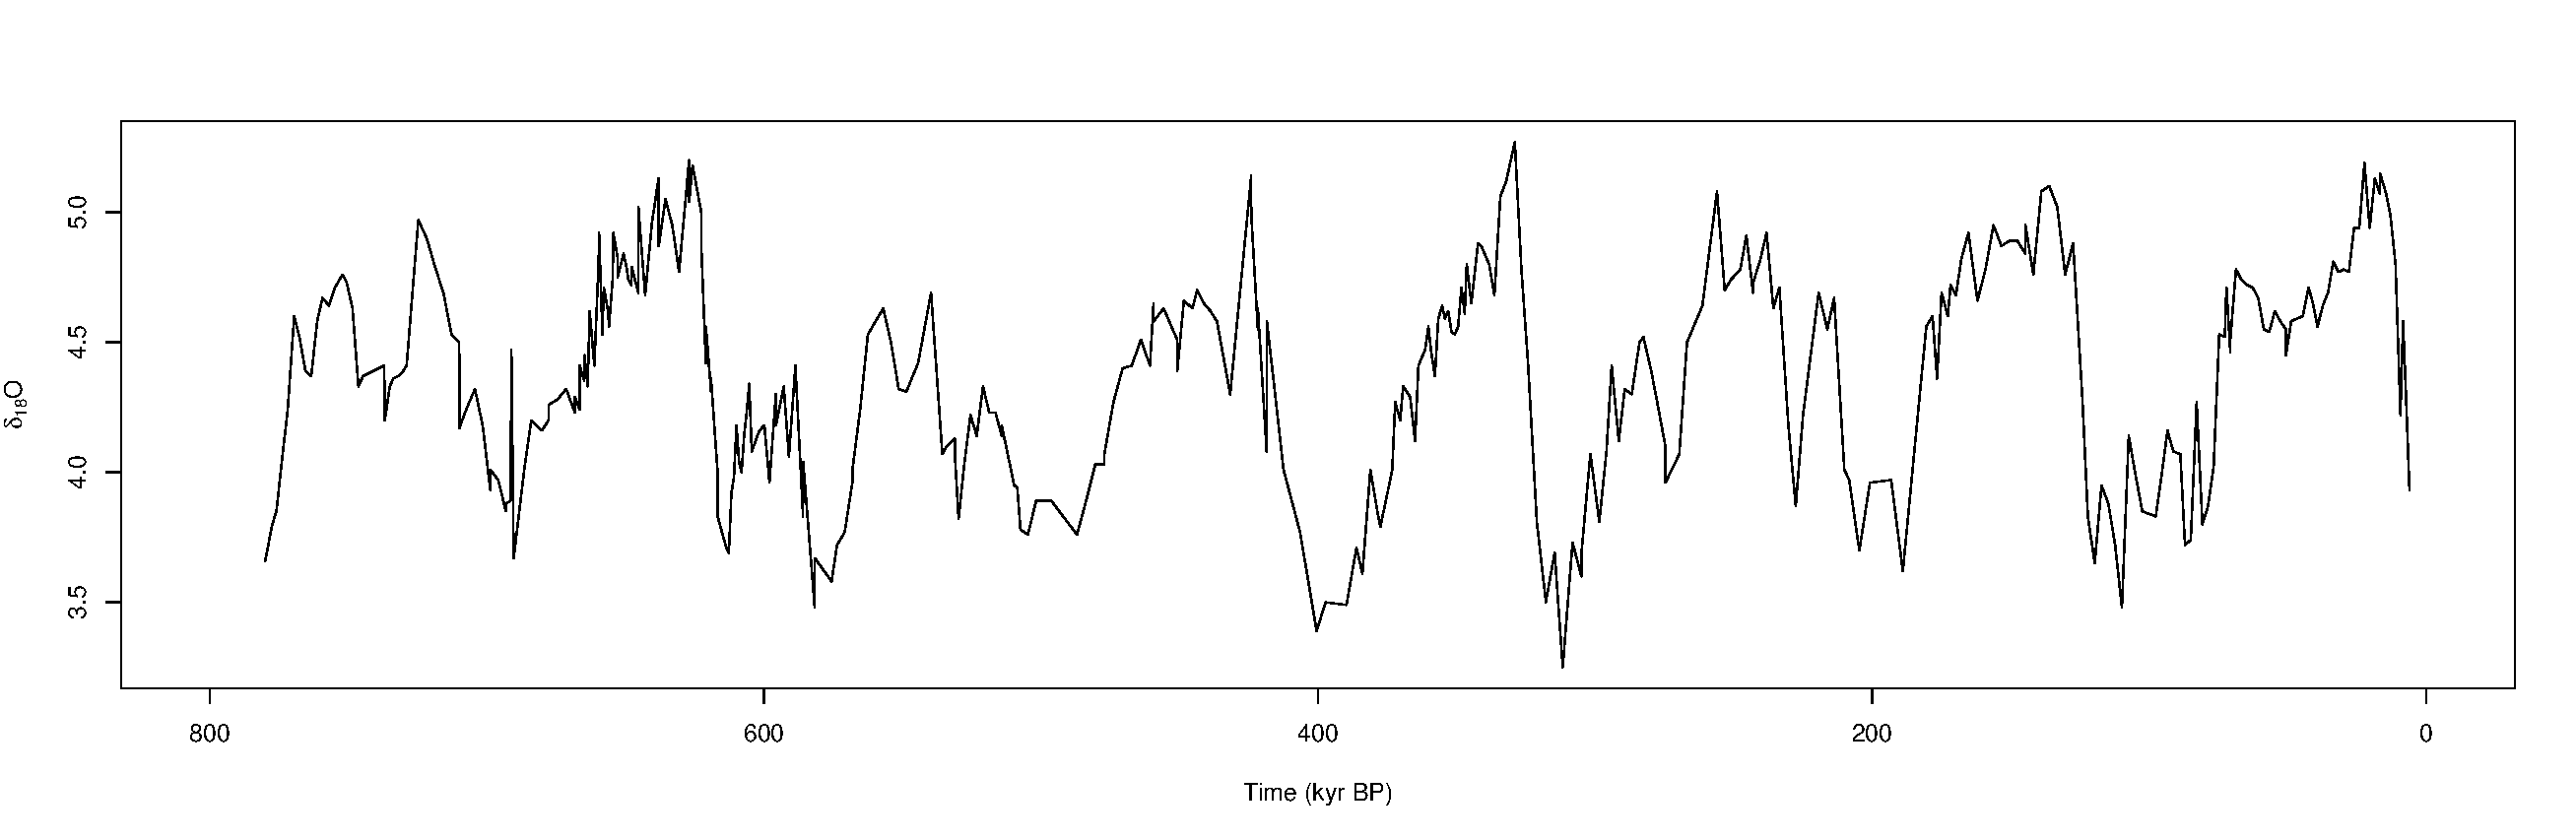
\includegraphics[width=\textwidth]{ODP677Plot.pdf}
\caption{
JAKE - Please can you make the axis labels larger?
Observed $\delta^{18}\mbox{O}$ from ODP677 \cite{Shackleton1990} corresponding to the past 780 kyr.
This dataset has been dated without the use of orbital tuning  \cite{Huybers2007}.}
\label{Fig:Data}
\end{figure}



\clearpage

\begin{figure}
\centering
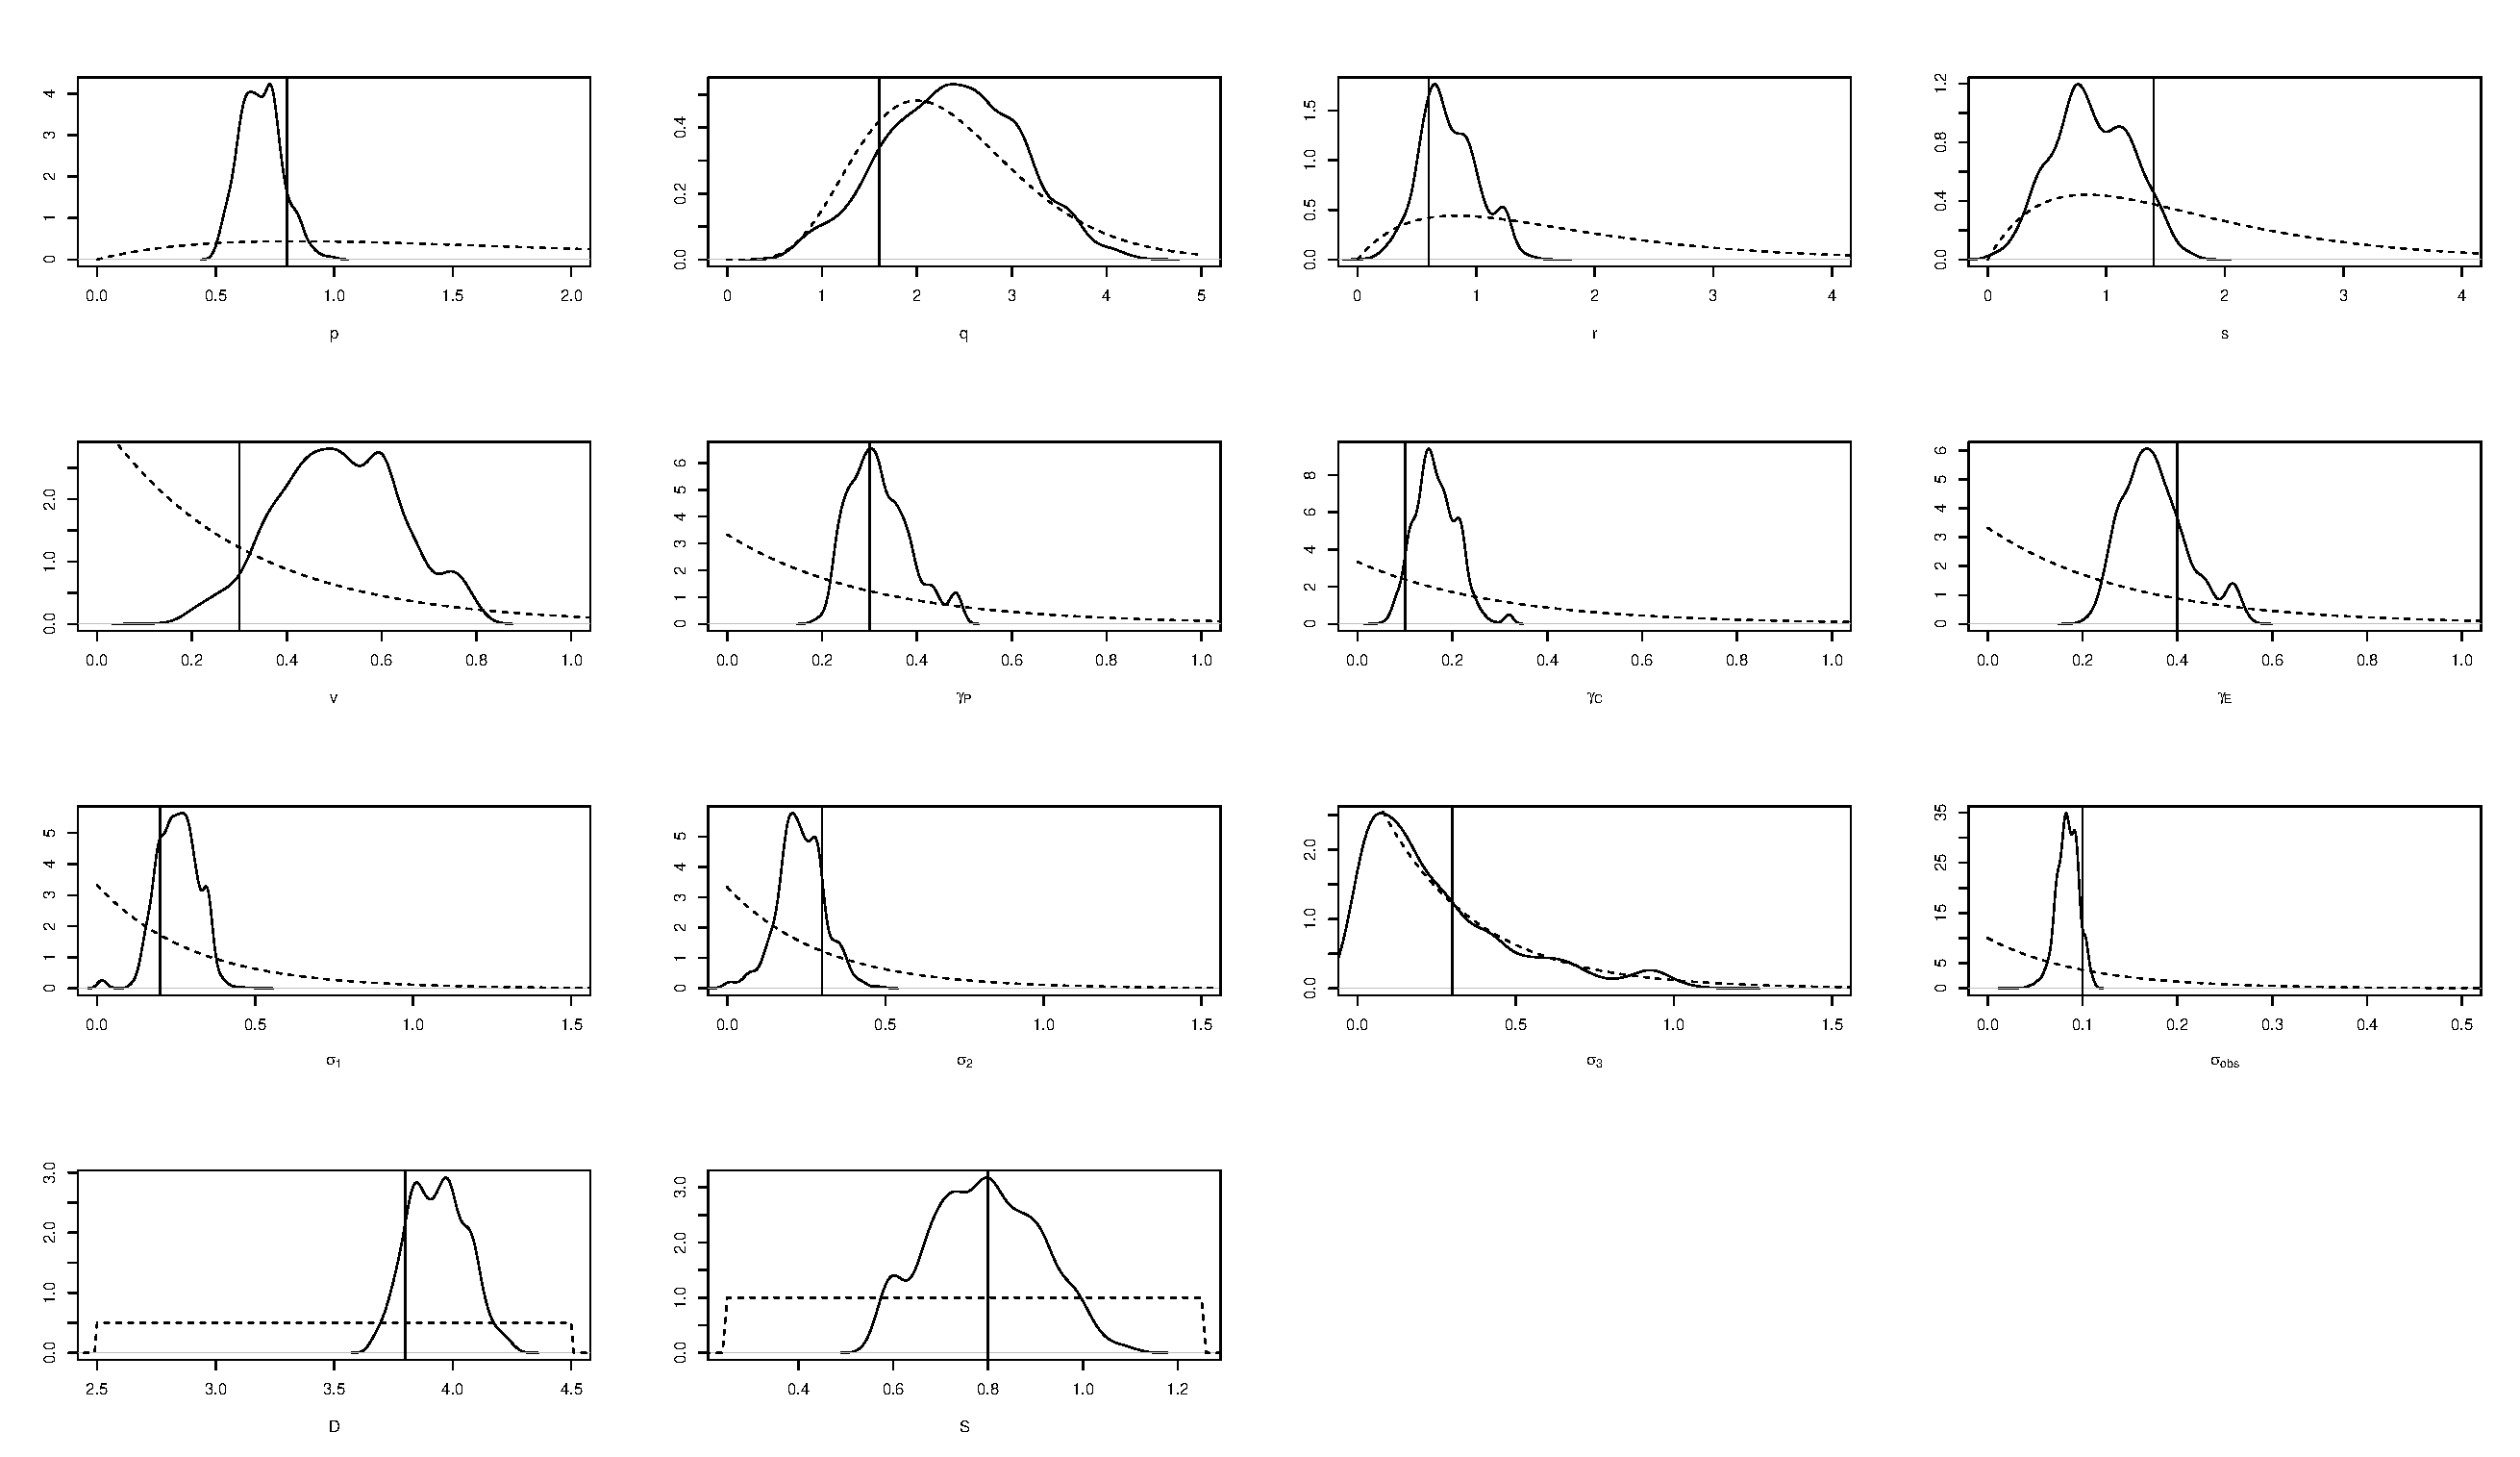
\includegraphics[width=\textwidth]{MSSSPE.pdf}\\\vspace{24pt}
\caption{
JAKE - Please can you make the axis labels larger?
Marginal posterior distributions for the parameters of the forced SM91 model when fit to the  SM91-f dataset.
Vertical lines show the parameter values used to generate the data, and dashed lines represent the prior distribution. 
}
\label{Fig:PosteriorSS}
\end{figure}


\clearpage

\begin{figure}
\centering
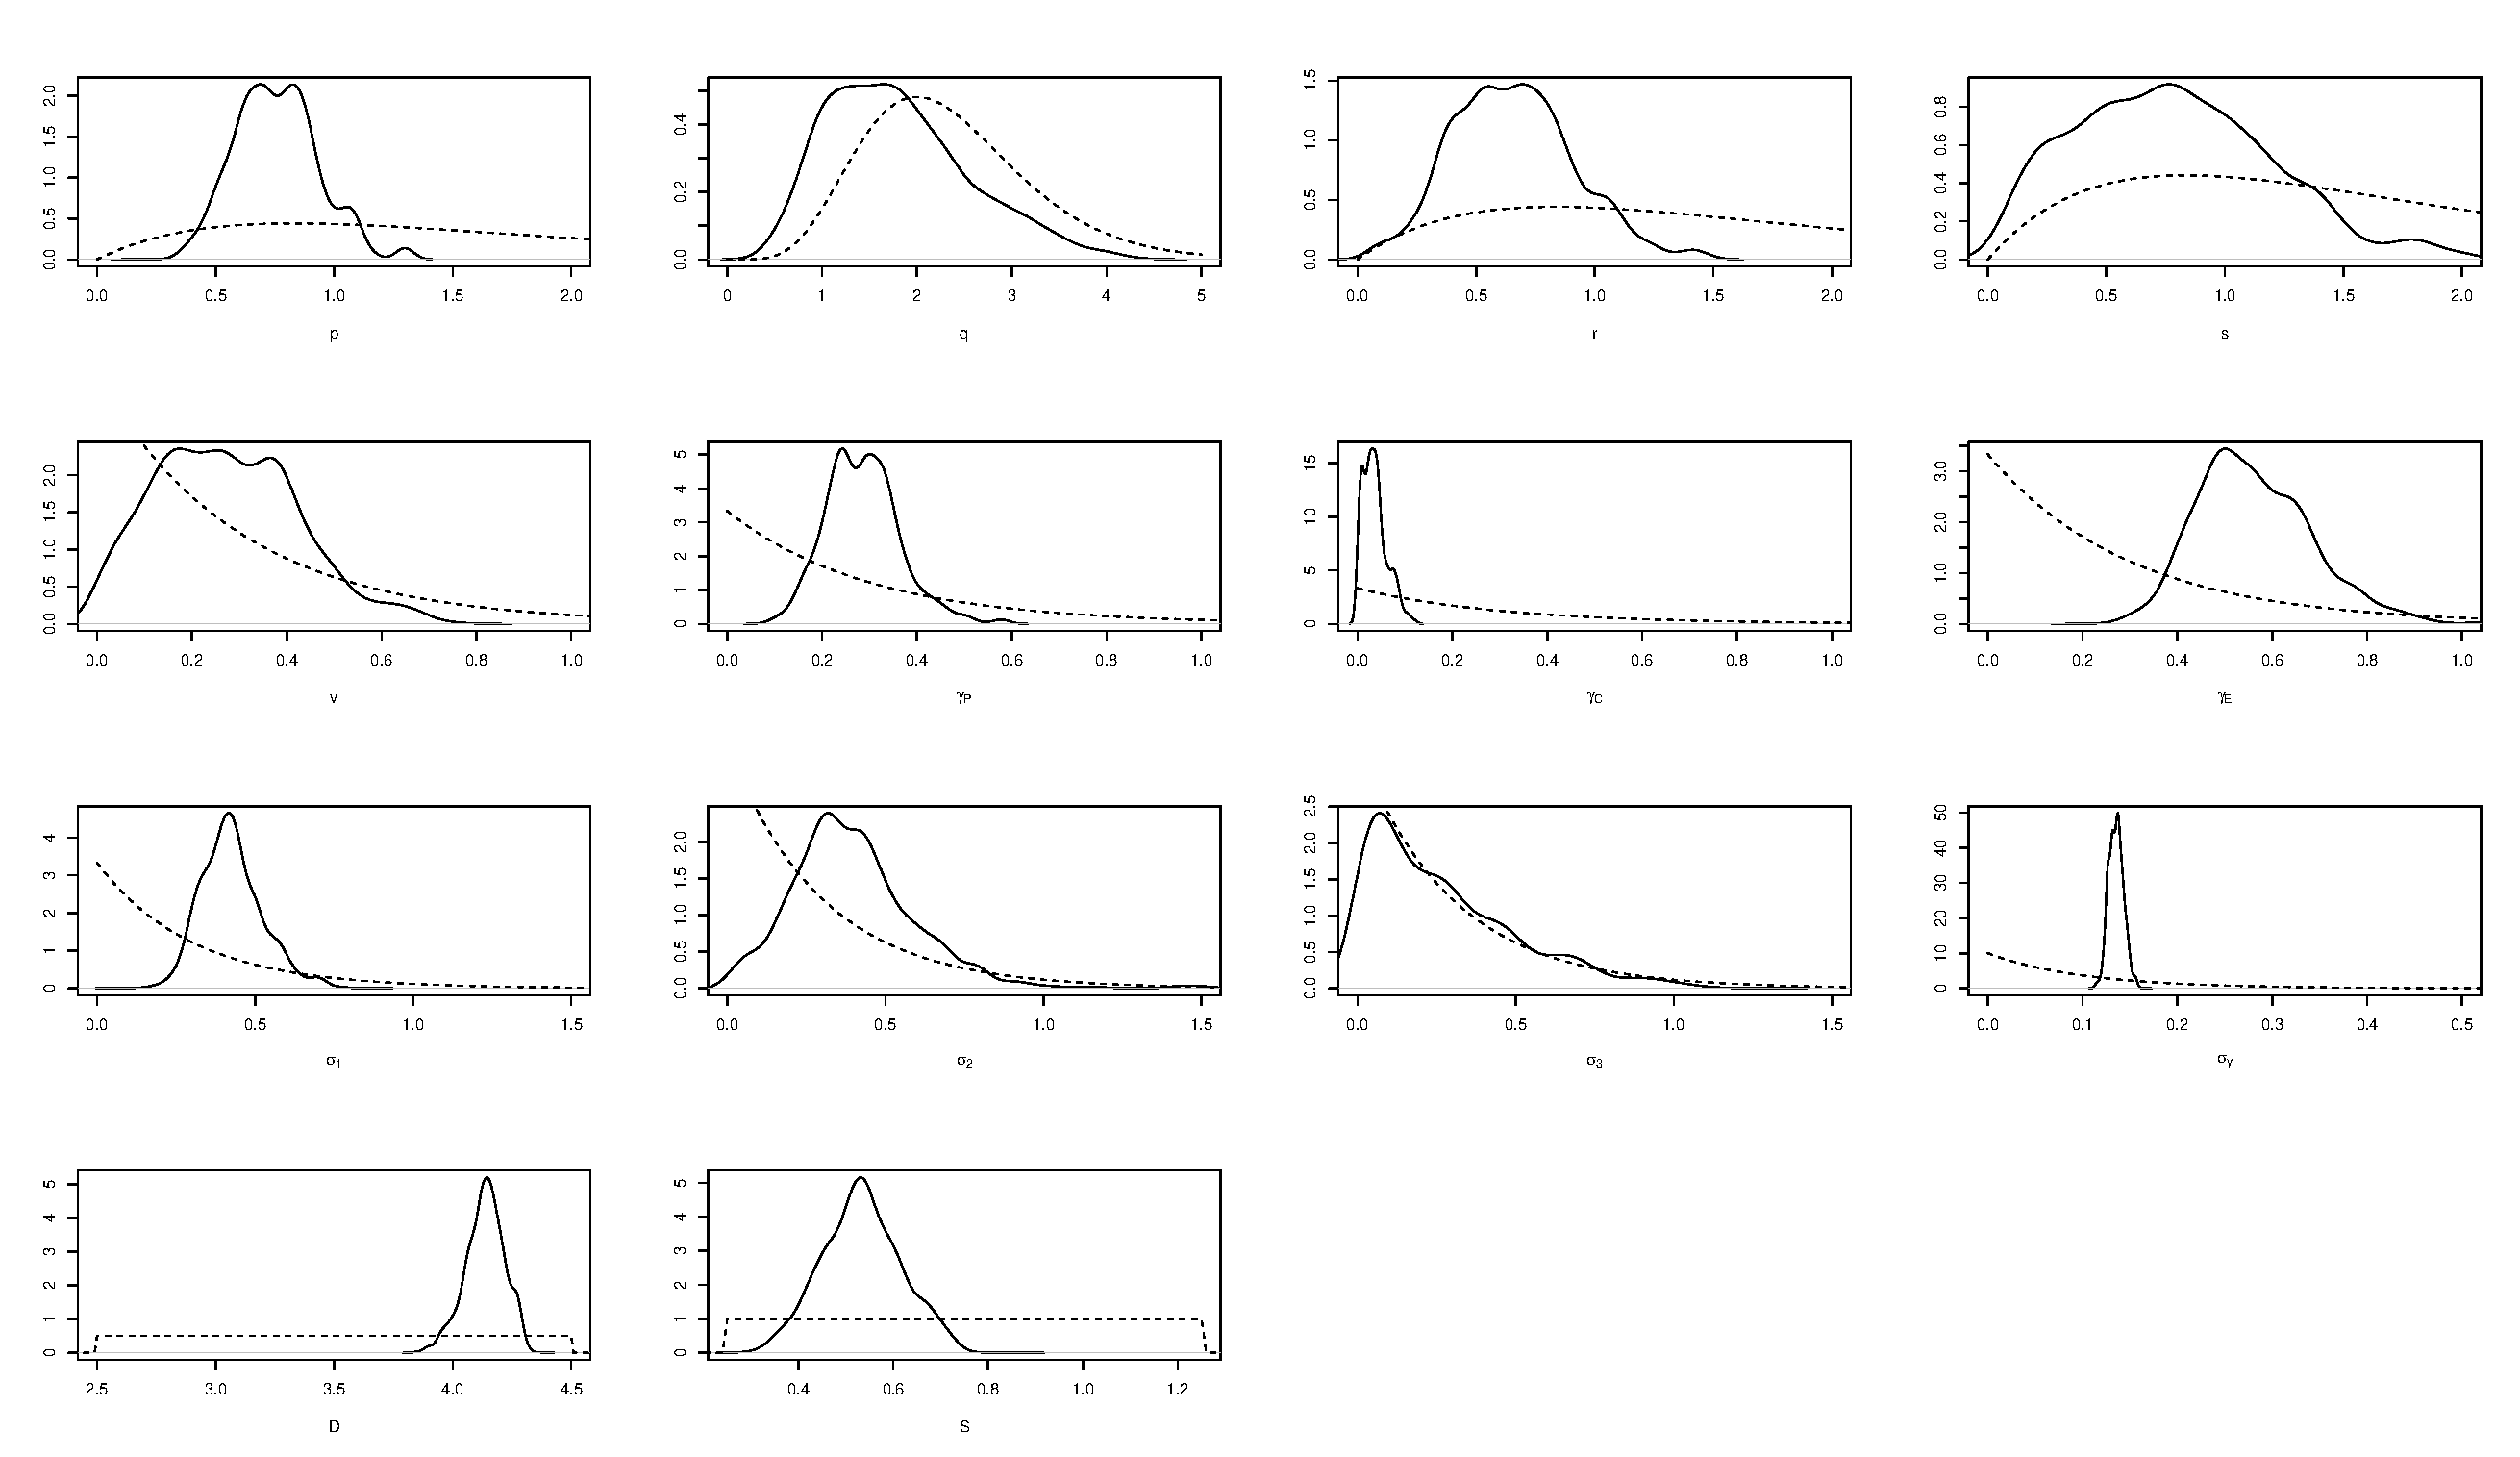
\includegraphics[width=\textwidth]{LR04677SM91.pdf}
\caption{
JAKE - Please can you make the axis labels larger?
Marginal posterior distributions for the fully forced SM91 model on ODP677-f. Dashed lines represent the prior distributions, and solid lines the posteriors. 
The prior distributions used are given in Table ref{Tab:Priors}}
\label{Fig:PosteriorODP}
\end{figure}



\clearpage

\begin{figure}
\centering
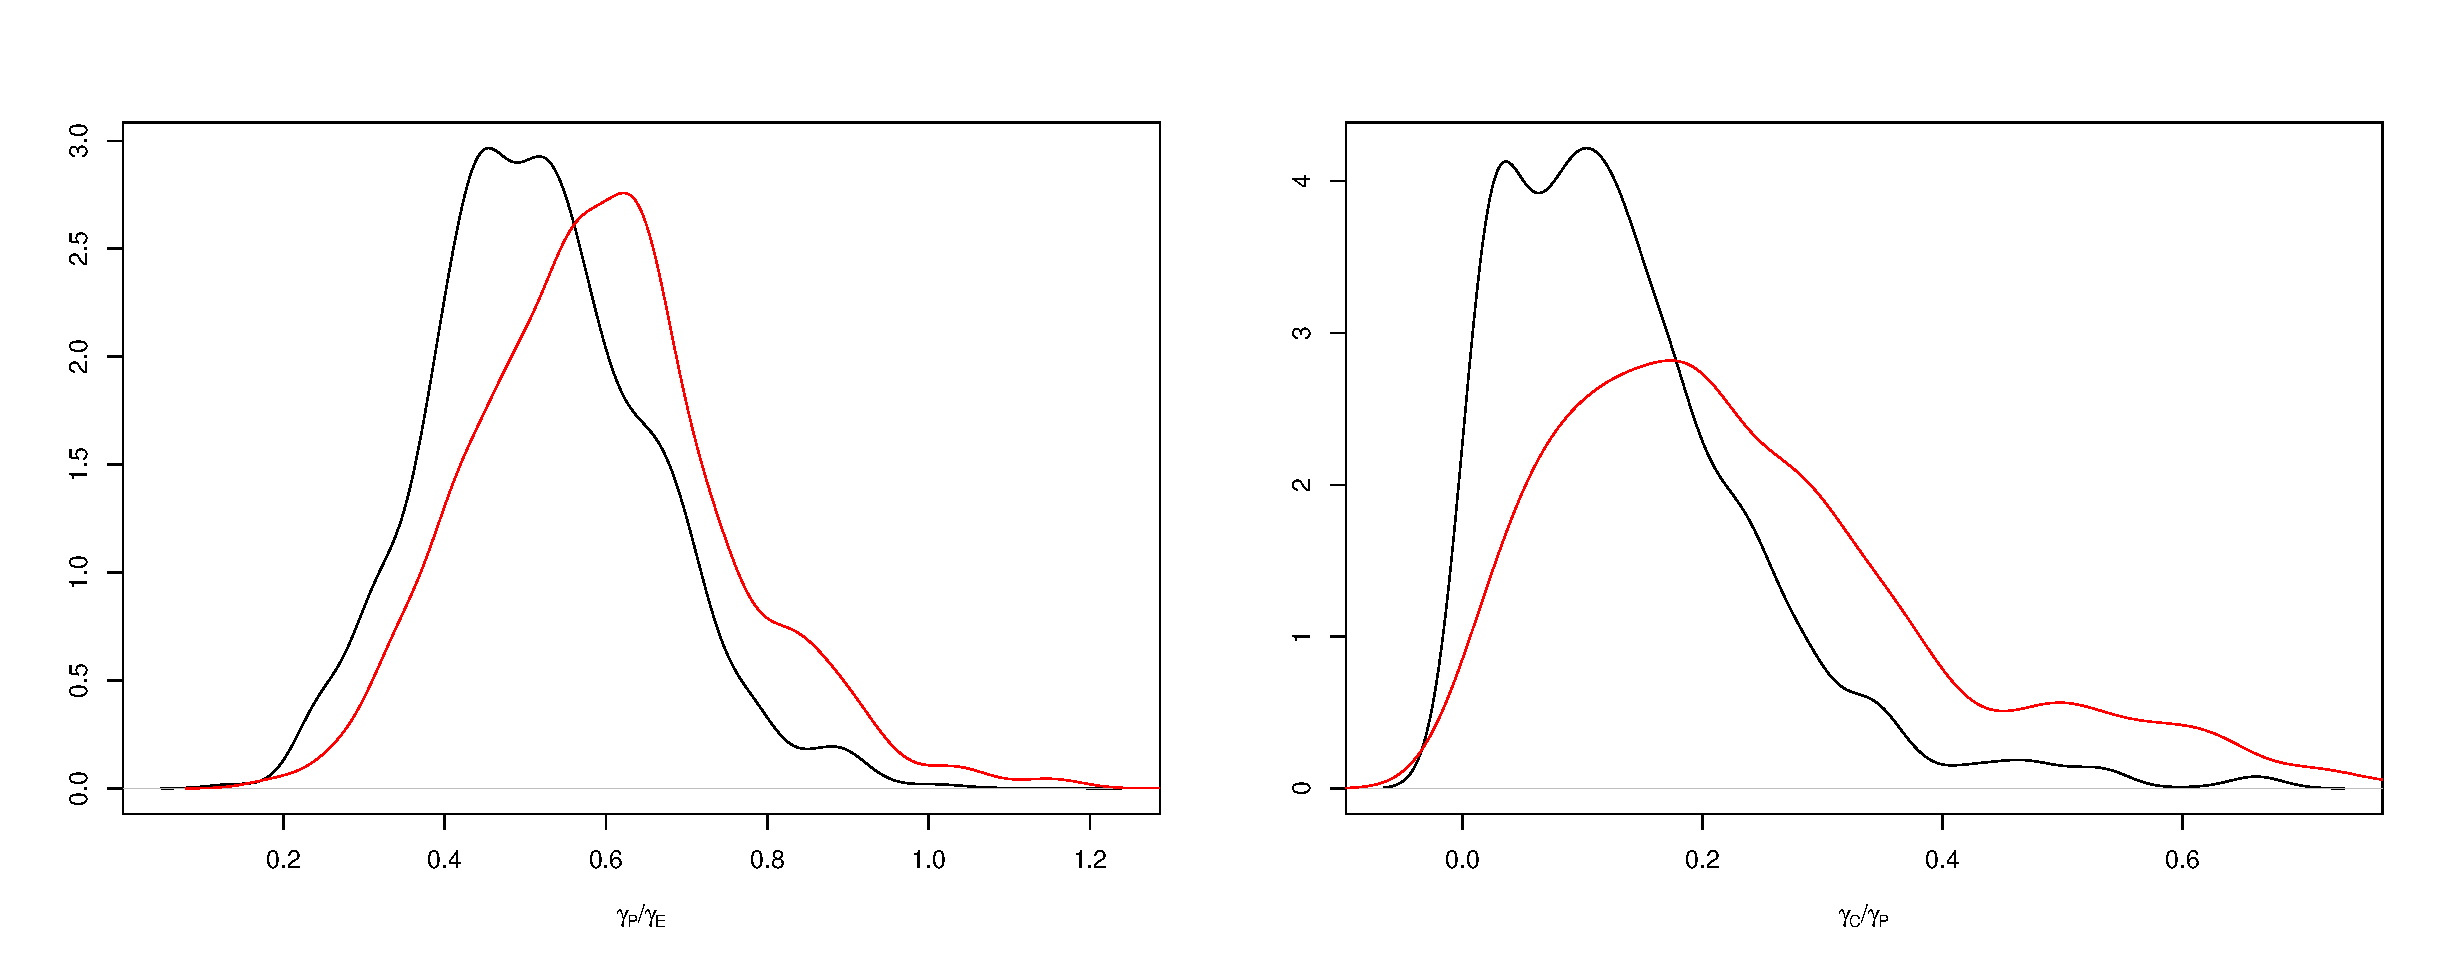
\includegraphics[width=\textwidth]{ForcingComparison.pdf}
\caption{
JAKE - Please can you make the axis labels larger?
Posterior density plot of the ratio of the orbital scaling terms for the SM91 model (black line), and T06 model (red line).}
\label{Fig:AFRatio}
\end{figure}


\clearpage

\begin{figure}
\centering
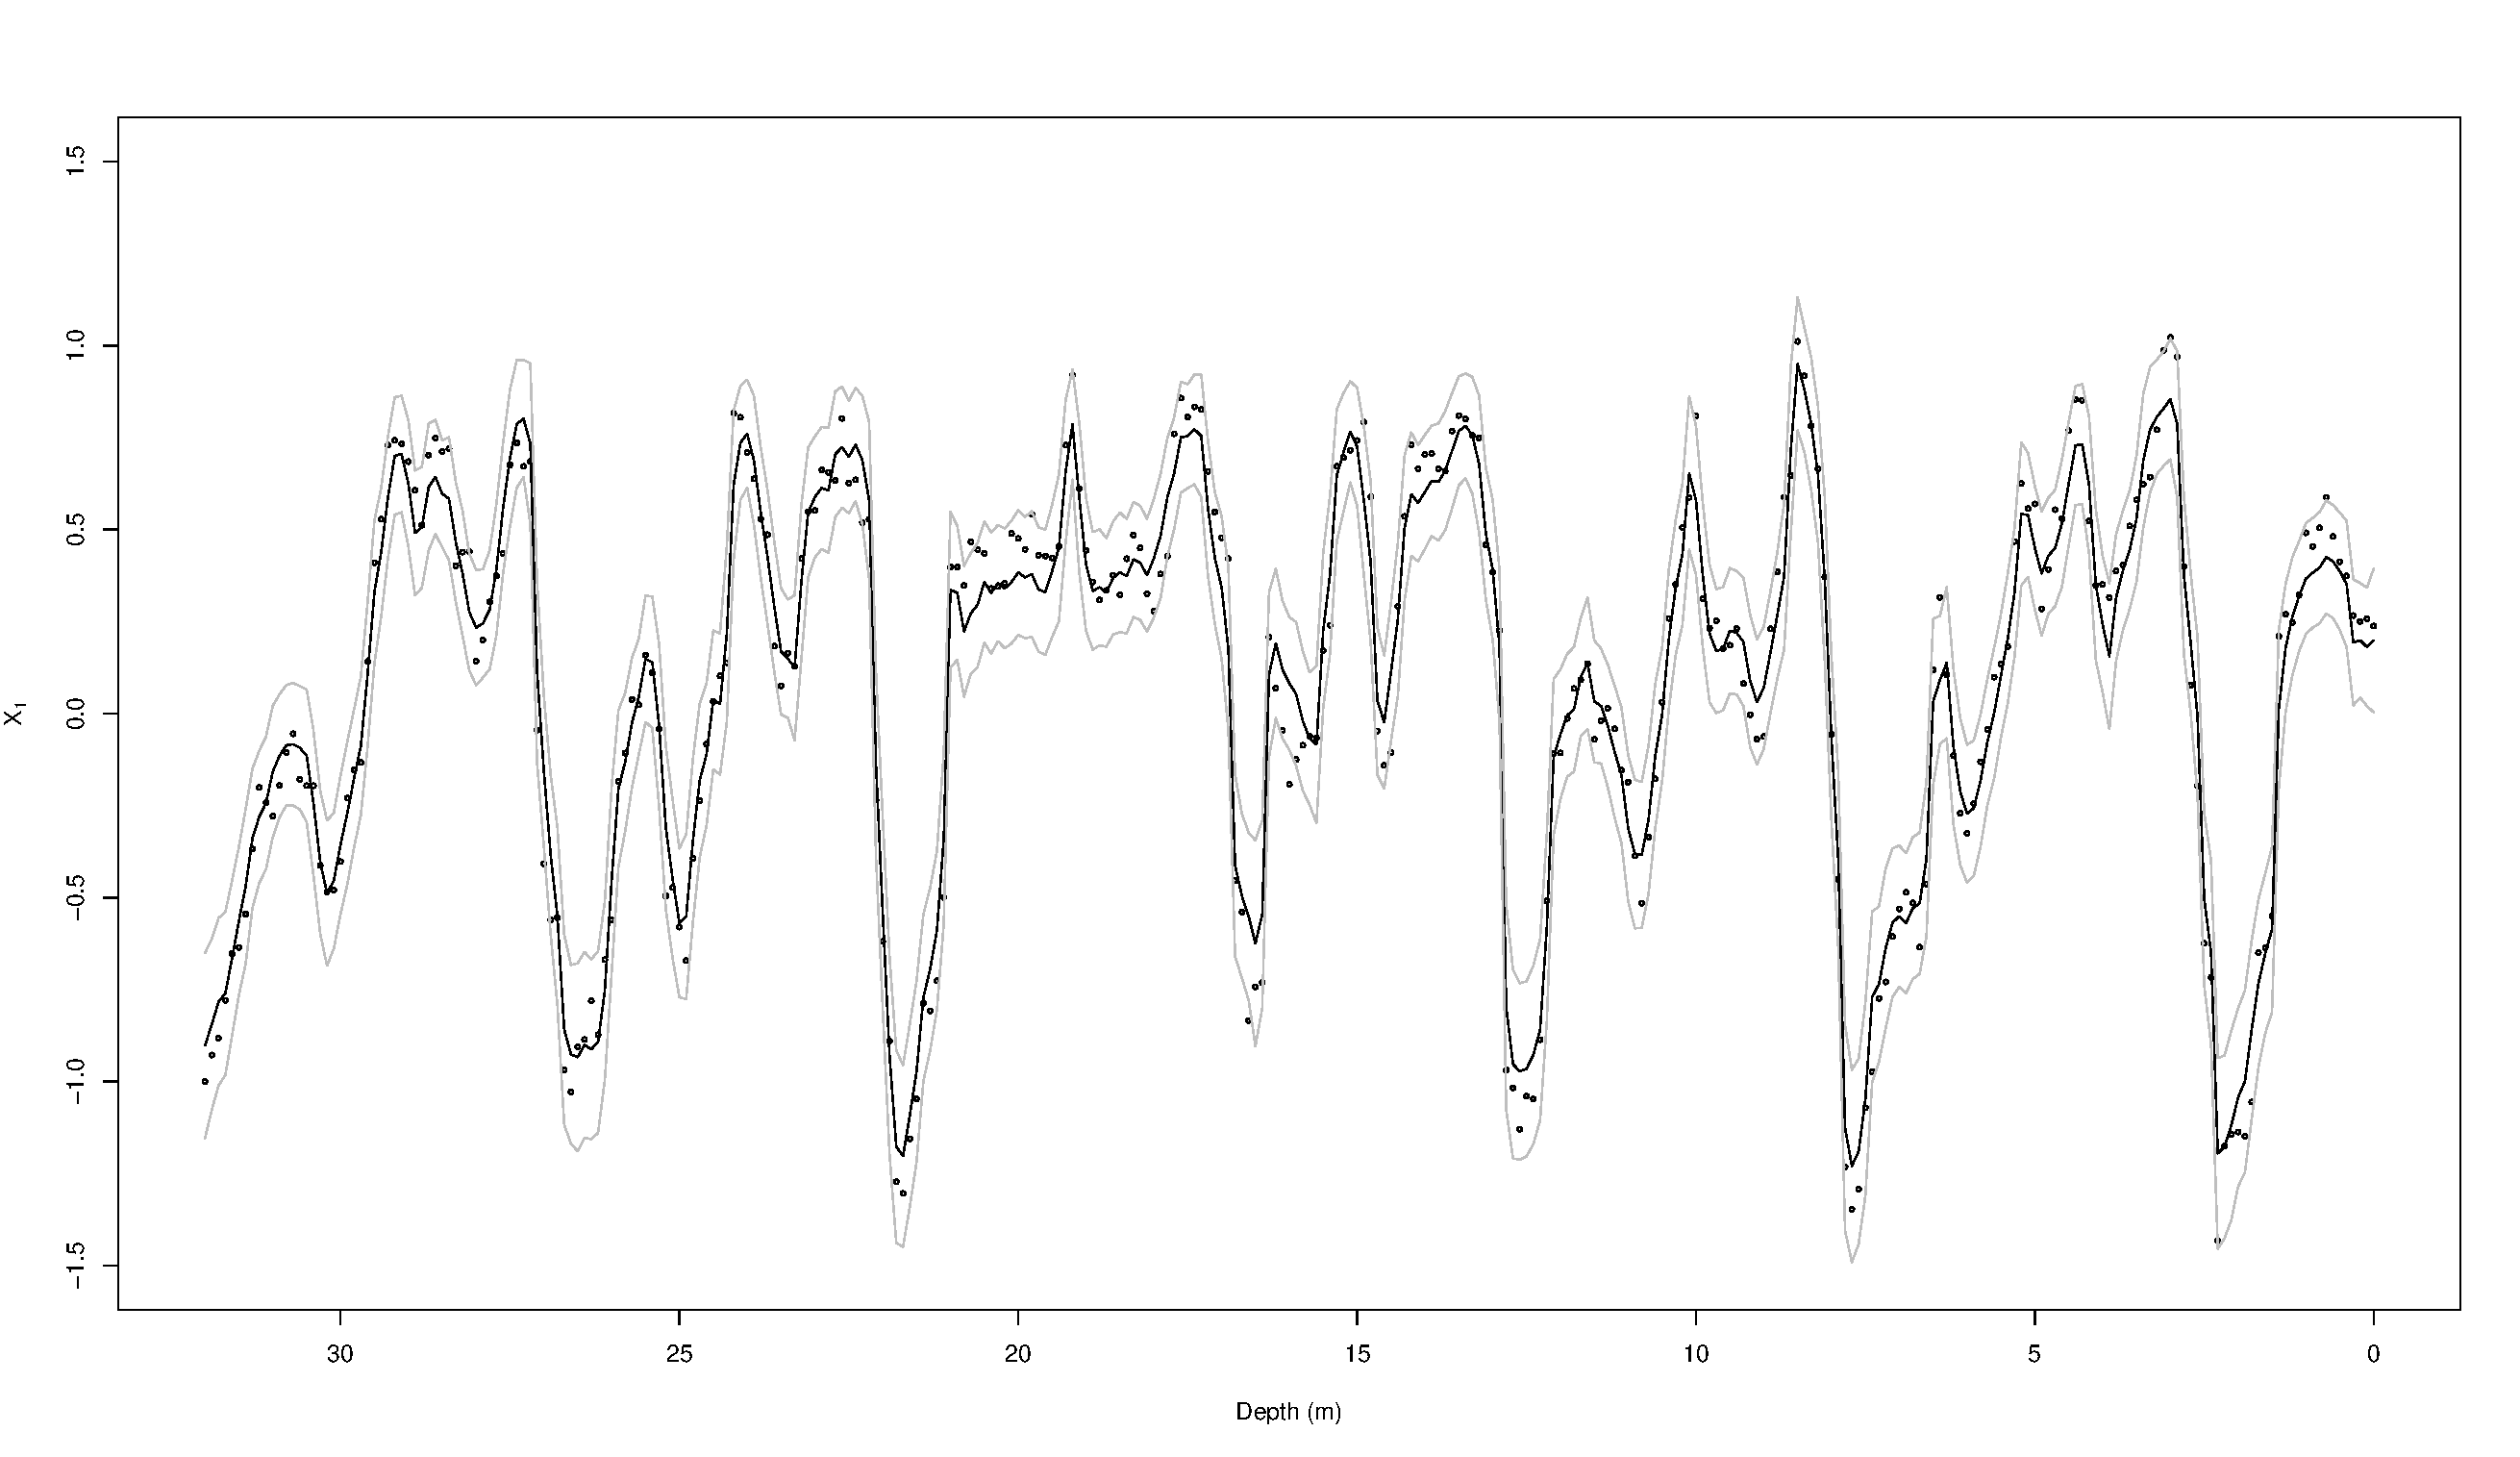
\includegraphics[scale=0.15]{CompactionSS01X01.pdf}\\
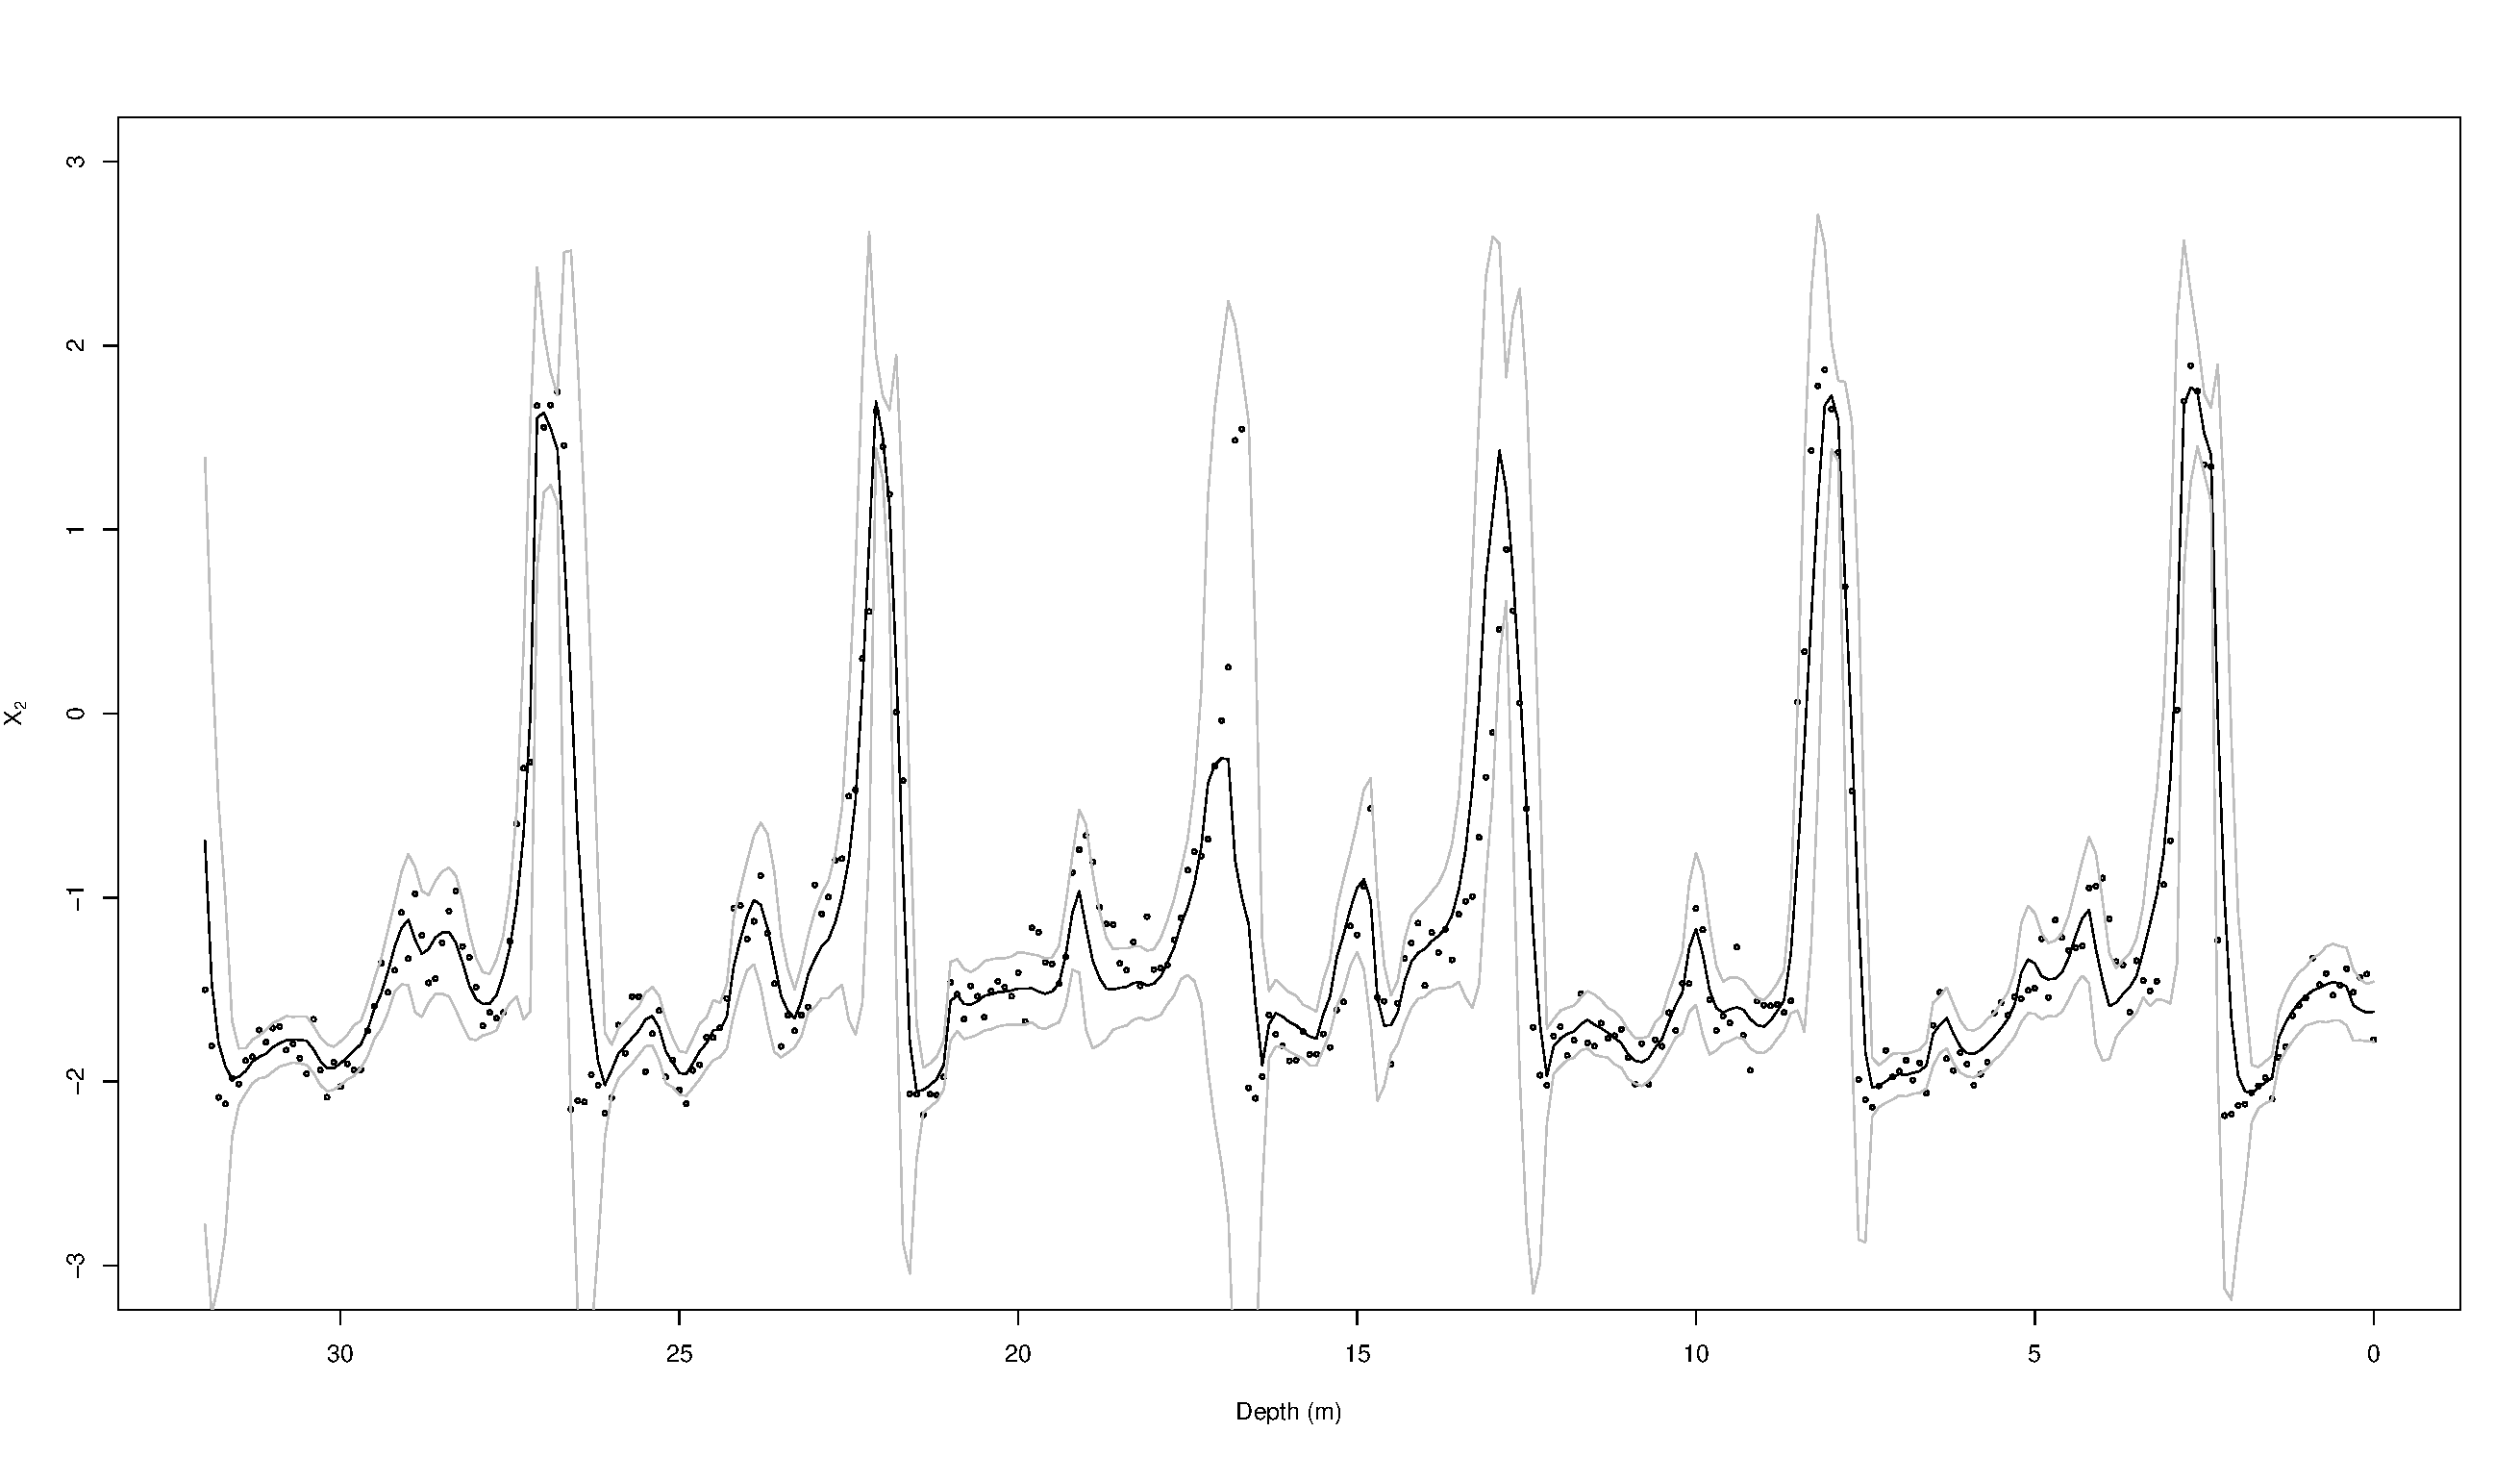
\includegraphics[scale=0.15]{CompactionSS01X02.pdf}
\caption{JAKE: These are the wrong figures - could you put in the correct figure. Add the truth on, and the data on $x_1$.   }
\label{Fig:Trajectories}
\end{figure}


%
%\begin{table}[t]
%\begin{center}
%\begin{tabular}{| l l | c c | c c |}
%
%\hline
%\multicolumn{2}{|c|}{Model} & \multicolumn{4}{|c|}{Evidence} \\
%\cline{3-6}
%& & SM91-u & SM91-f & ODP677-u & ODP677-f\\
%\hline
%SM91 & Forced & $5.6 \times 10^{28}$ & $1.4 \times 10^{41}$ & $4.0 \times 10^{24}$ & $1.1 \times 10^{28}$ \\
% & Unforced & $1.1 \times 10^{30}$ & $2.4 \times 10^{18}$ & $3.5 \times 10^{26}$ & $1.6 \times 10^{18}$ \\
%T06 & Forced & $3.6 \times 10^{20}$ & $2.6 \times 10^{30}$ & $3.3 \times 10^{25}$ & $4.5 \times 10^{29}$  \\
% & Unforced & $1.1 \times 10^{22}$ & $2.9 \times 10^{14}$ & $1.7 \times 10^{28}$ & $3.3 \times 10^{21}$  \\ 
%PP12 & Forced & $2.8 \times 10^{8}$ & $2.1 \times 10^{18}$ & $1.5 \times 10^{22}$ & $1.8 \times 10^{34}$  \\
%\hline
%\end{tabular}
%\caption{The model evidence for each model over different datasets.}
%\label{Tab:Evidence}
%\end{center}
%\end{table}
%




\end{document}
